% Chapter Template

\chapter{Memristor Simulation} % Main chapter title

\label{Chapter5} % Change X to a consecutive number; for referencing this chapter elsewhere, use \ref{ChapterX}

\lhead{Chapter 5. \emph{Memristor Simulation}} % Change X to a consecutive number; this is for the header on each page - perhaps a shortened title

A numerical method for a memristor simulation was developed and tested in previous chapters based on drift-diffusion equations and finite difference. This chapter introduces the memristor's structure and physical parameters used for the simulation. It continues with a preliminary problem analysis to determine required mesh density and maximum possible time step. This preliminary analysis is followed by 1-D simulations of 3 different cross sections of a memristor.

\section{Memristor Structure}
%-Problem Analysis and assumptions, semiconductor vs memristor plots
Following figure (\ref{MemStc}) shows the structure of a simple memristor which will be taken as a basis for all the memristor simulations presented in this thesis. It consists of 2 metal contacts a polymer conductor (PEDOT:PSS) and an electrolyte solution which has lithium and perchlorate ions (6.02 $10^{26} m^{-3}$). The memristor is about 1 cm long. The thickness of the conductive layer is around 1 $\mu$m. During experimentation the electrolyte is deposited on PEDOT via a syringe so its thickness can vary drastically but as long as the amount of ions in the electrolyte solution is enough to saturate PEDOT this does not make a significant difference in the operation of the memristor. For simulation it was assumed that there were always more than enough ions to saturate the PEDOT so the electrolyte was modeled as an infinite source/sink of ions. The top boundary of the electrolyte was assumed to be charge neutral at all times which provides a mechanism for moving ions in and out of the system. This way the movement of ions near the surface of the PEDOT can still be captured without having to simulate the ion movement for the entire electrolyte solution which is variable in size. 

\begin{figure}[!htp]
\centering
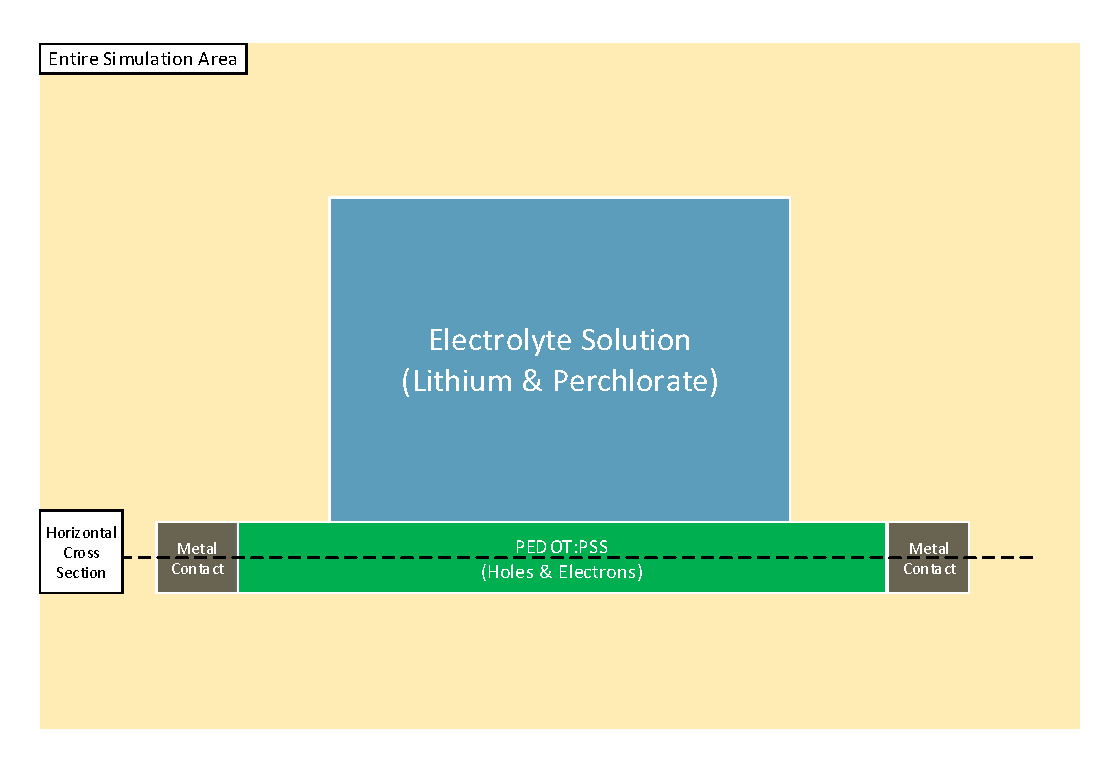
\includegraphics[scale=0.50]{Mem1}
\caption{} 
\label{MemStc}
\end{figure}

The initial conditions for all the charge carriers are the same. All charge are balanced and uniformly distributed but the carrier density in the electrolyte solution is higher than the carrier density in PEDOT. Perchlorate ions are not allowed to move outside the electrolyte solution so a no flow boundary condition was used around the electrolyte. Lithium ions are free to move between PEDOT and the electrolyte solution but their maximum concentration is limited inside the PEDOT. The mobility of lithium ions has further restrictions inside PEDOT. Lithium has higher mobility in region of PEDOT under the electrolyte solution, wet PEDOT, than the region without any contact with electrolyte, dry PEDOT. In fact due to this difference very little amount of lithium reaches the metal contacts. This decrease in mobility was modeled by making the mobility of lithium a function of position. The mobility of lithium ions were assumed to be 100 times slower than the mobility of holes ( $\approx$ $10^{-4}$ $m^2/Vs$).  

PEDOT:PSS is a regular conductor with fixed negative charge and mobile holes. Holes can move in an out of the PEDOT through the metal contacts which hold the charge neutrality of the initial condition throughout the simulation. The interface between PEDOT and electrolyte only allows the exchange of lithium ions. During simulation,the movement of lithium ions changes the conductivity of the PEDOT by increasing or decreasing the amount of available holes through coulomb forces. In the actual device lithium ions change the conductivity via various physical effects like changing the mobility of holes through modifying their hopping distance. These additional affects are beyond the scope of this thesis. 


\clearpage
\section{Simulation Requirements}

It is important to analyze computational requirements of a simulation in order to asses the feasibility of the computation scheme. It is possible to determine these spacial and temporal requirements using the equations \ref{debye} to \ref{CFL_Drift} which describe physical and numerical limitations of the simulation. Following graph \ref{SpaceTime} shows the requirements for a memristor of the scale discussed above and a typical semiconductor device around 1 $\mu$m. The mesh density has to be high enough in order to capture the exponential charge accumulation for charge shielding so the minimum step size was set to be 5 times the Debye length. Plots \ref{SpaceTime}.a and \ref{SpaceTime}.c show the amount of points required to simulate a semiconductor and a memristor based on minimum step size. It is important to note that these values are for 1-D simulation and they can be converted to 2-D and 3-D by squaring or cubing y axis values respectively. Plots \ref{SpaceTime}.b and \ref{SpaceTime}.d were created using CFL conditions for drift and diffusion and dielectric relaxation time. A typical simulation time was estimated using mobility and electric field. Based on the estimated simulation time the number of time steps were calculated using the minimum time step obtained from CFL conditions and dielectric relaxation time.

It can be seen from graphs \ref{SpaceTime}.a and \ref{SpaceTime}.c that memristor simulations require much higher mesh densities compared to a typical semiconductor simulation. This is due to the larger size and higher charge density of the memristor. Graph \ref{SpaceTime}.a \ref{SpaceTime}.b show that a memristor with $10^{26}$ $m^{-3}$ charge density of the electrolyte would require close to $10^9$ points and $10^{14}$ time steps to simulate in 1-D. These requirements make the simulation of the memristor extremely challenging. One possible solution to this problem is to use a much lower charge density and assume that all the values scale linearly. Following cross sectional simulations (Figure \ref{MemStc}) were made to determine the effect of increasing charge density on memristor simulations and to investigate if scaling can be used without compromising the reliability of the simulation.

\begin{landscape}
\begin{figure}[htp]
\centering
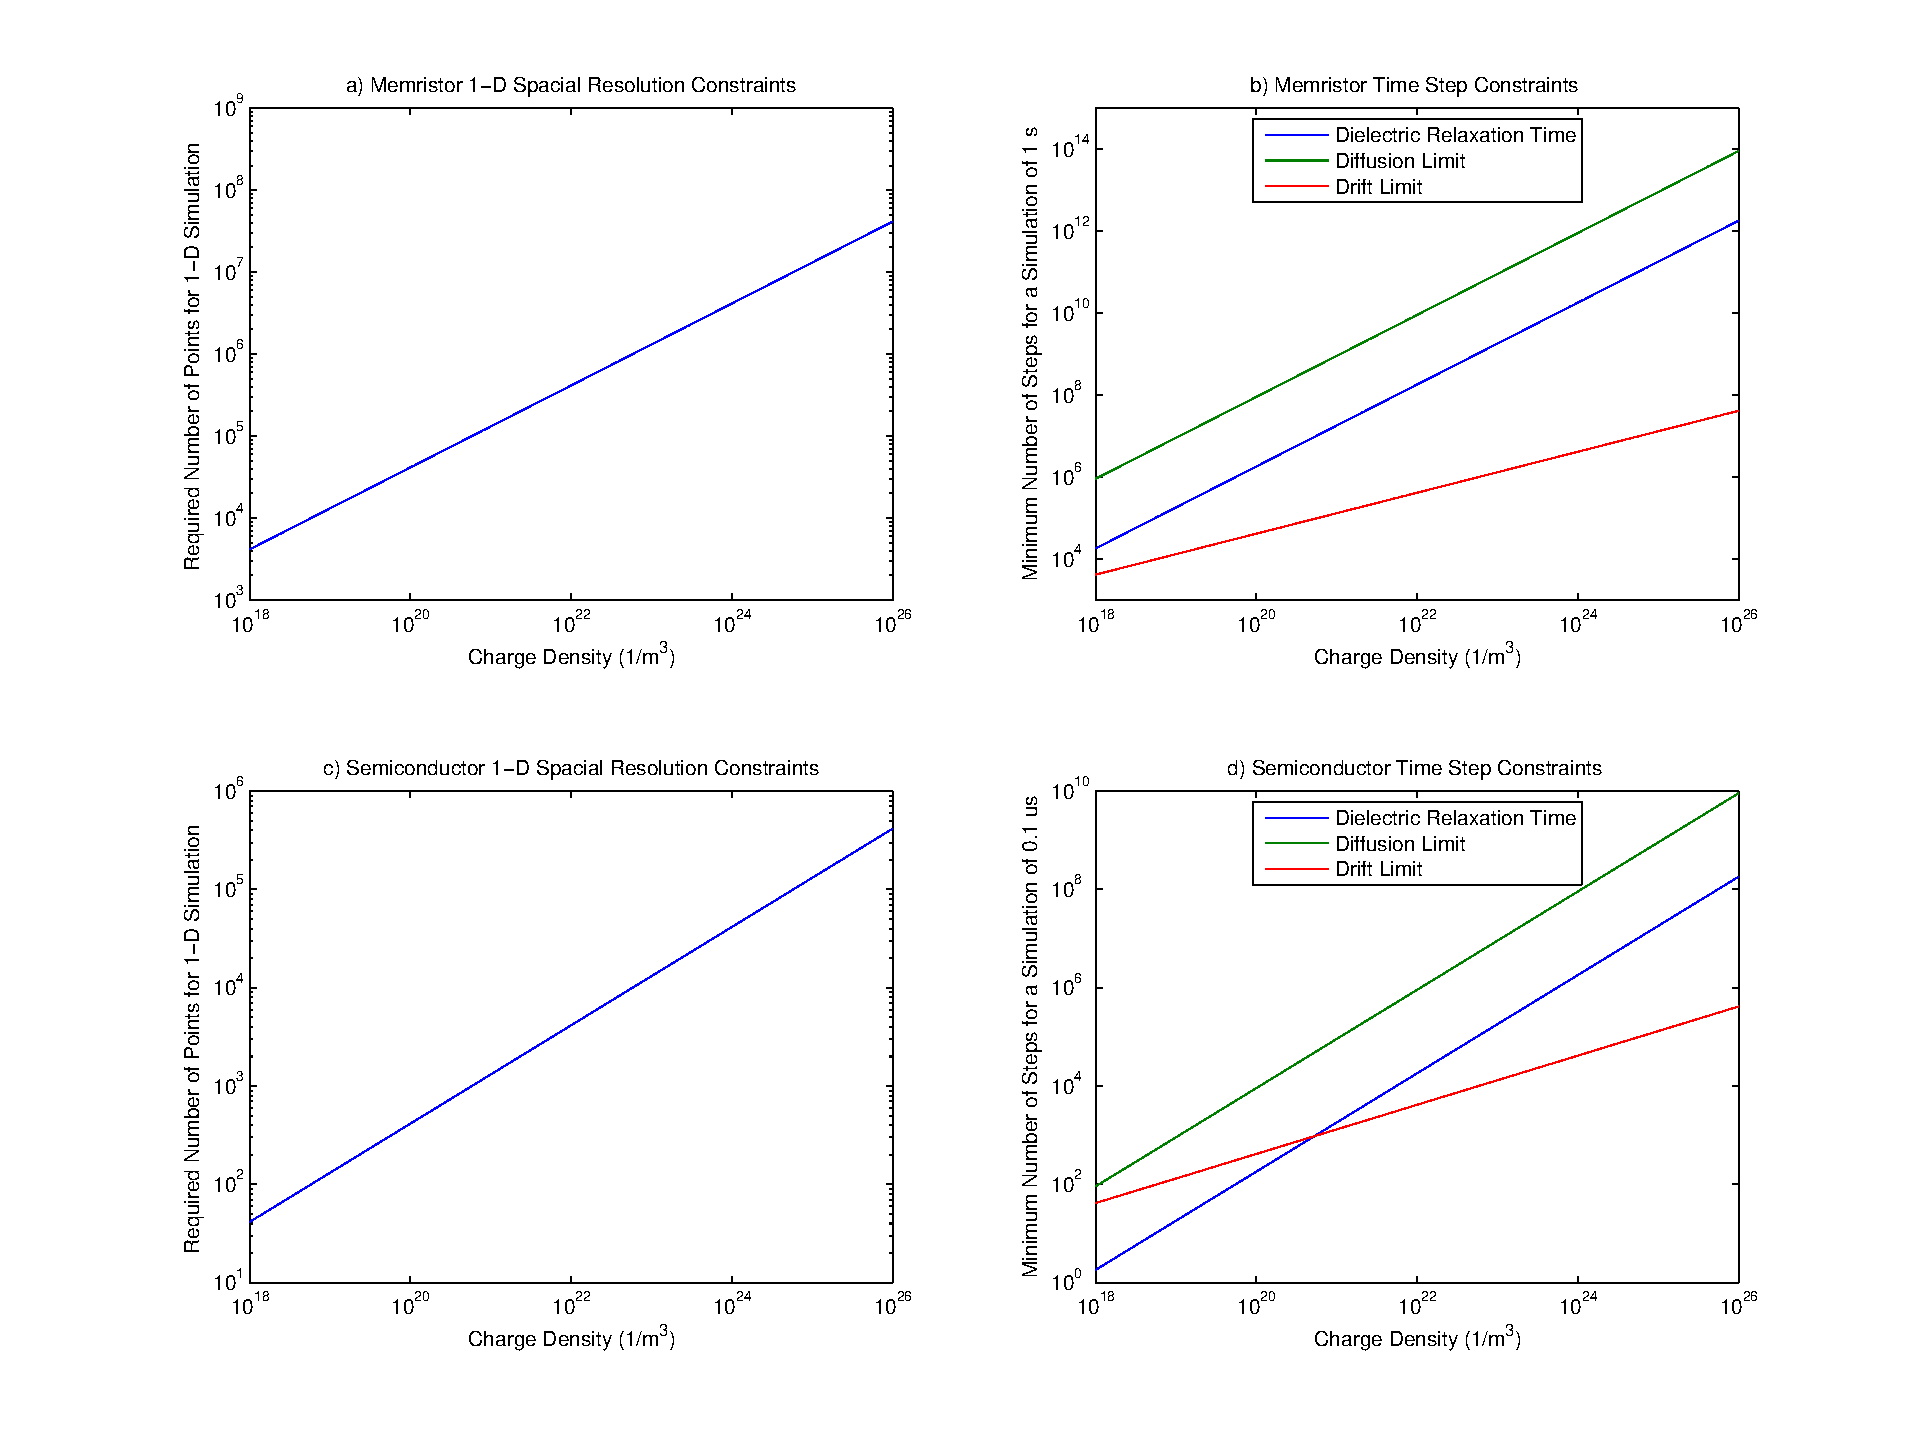
\includegraphics[scale=0.60]{SpaceTime}
\caption{Spatial and temporal requirements for simulation} 
\label{SpaceTime}
\end{figure}
\end{landscape}

\clearpage
\section{Memristor Cross Sectional Simulations}

Even though it is possible to simulate the structure presented in section 5.1 in 2-D, simulating cross sections of the memristor separately has a major advantage. The purpose of these preliminary  simulations is to test the affect of various charge densities which requires mesh density to be as high as possible. Increasing mesh density in 1-D has a smaller impact on computational load therefore higher charge densities are more accessible.  

In following 1-D simulations initial carrier densities ranging from $2$ $10^{15}$ $m^{-3}$ to $10$ $10^{15}$ $m^{-3}$ were used. Unless otherwise stated the plots for charged particle densities were normalized to $2$ $10^{15}$ $m^{-3}$ in order to show the effect of density scaling. 

\subsection{Electrolyte Simulation (Cross Section 1)}

A steady state and transient solution of the cross section 1 indicated in figure \ref{MemStc} is presented in this section. Positive an negative charges were uniformly initialized at different densities for each simulation and two contacts representing the elctric field generated by the metal contacts of the memristor were placed on each side of the electrolyte. Potential on the metal contacts were kept at 1 V and 0 V on the left and right side respectively. The electrolyte solution has a high density of positive and negatively charged particles. As long as there are enough particles, any electric field inside the electrolyte will be canceled out due to separation of charge. This means that, in a memristor, any electric field due to metal contacts reaching the electrolyte will be canceled out. Following figure (\ref{ElectrolyteQ}) shows the distribution of net charge density in steady state for various initial charge densities.  These plots were not normalized since the net charge required to cancel the electric field is the same for all densities. Naturally, the final charge distribution is almost identical in all cases.

\begin{figure}[htp]
\centering
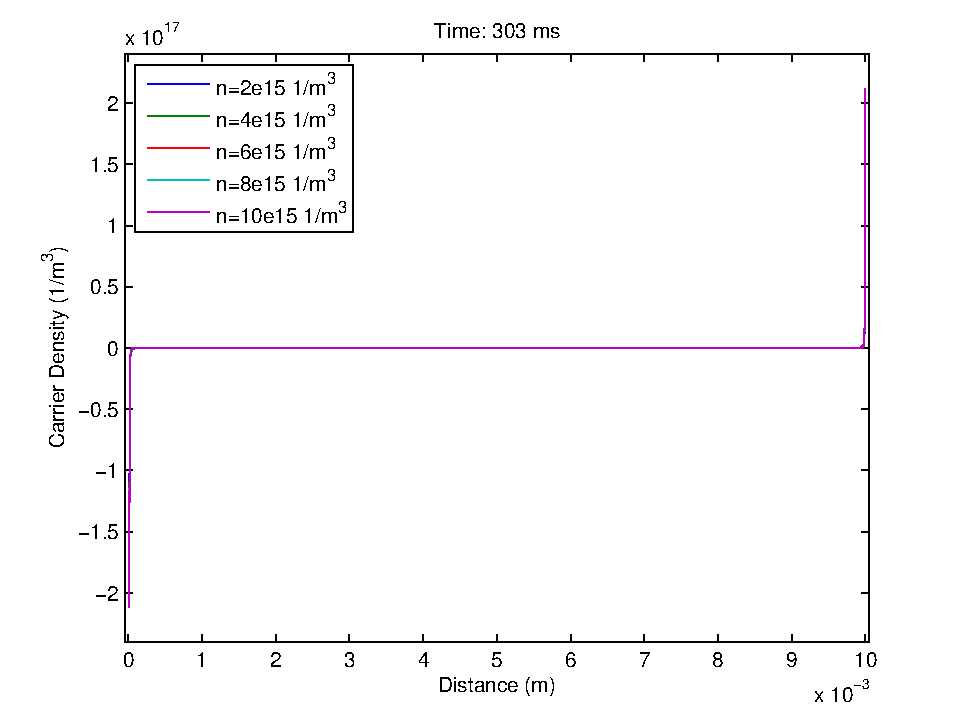
\includegraphics[scale=0.50]{Ex1NetQ_Time_All}
\caption{Final net charge density distribution in electrolyte subject to an electric field} 
\label{ElectrolyteQ}
\end{figure}

Figure \ref{ElectrolyteQzoom} shows the charge accumulation on the right wall over time. It can be seen that the higher the initial charge concentration is the faster it reacts to the applied field. This behavior is expected since with higher charge density less charge needs to move in order to cancel the electric field. This effect can better be seen in figure \ref{ElectrolyteV} which shows the evolution of potential over time. The change in potential over time shows that higher densities cancel out the electric field faster than lower densities.

The inverse relationship between charge density and debye length was given in equation \ref{debye} which can be physically be observed from figure  \ref{ElectrolyteV2}. The distance over which the potential is being canceled out is getting shorter with the increase of charge density.  

 
\begin{landscape}
\begin{figure}[!htp]
\centering
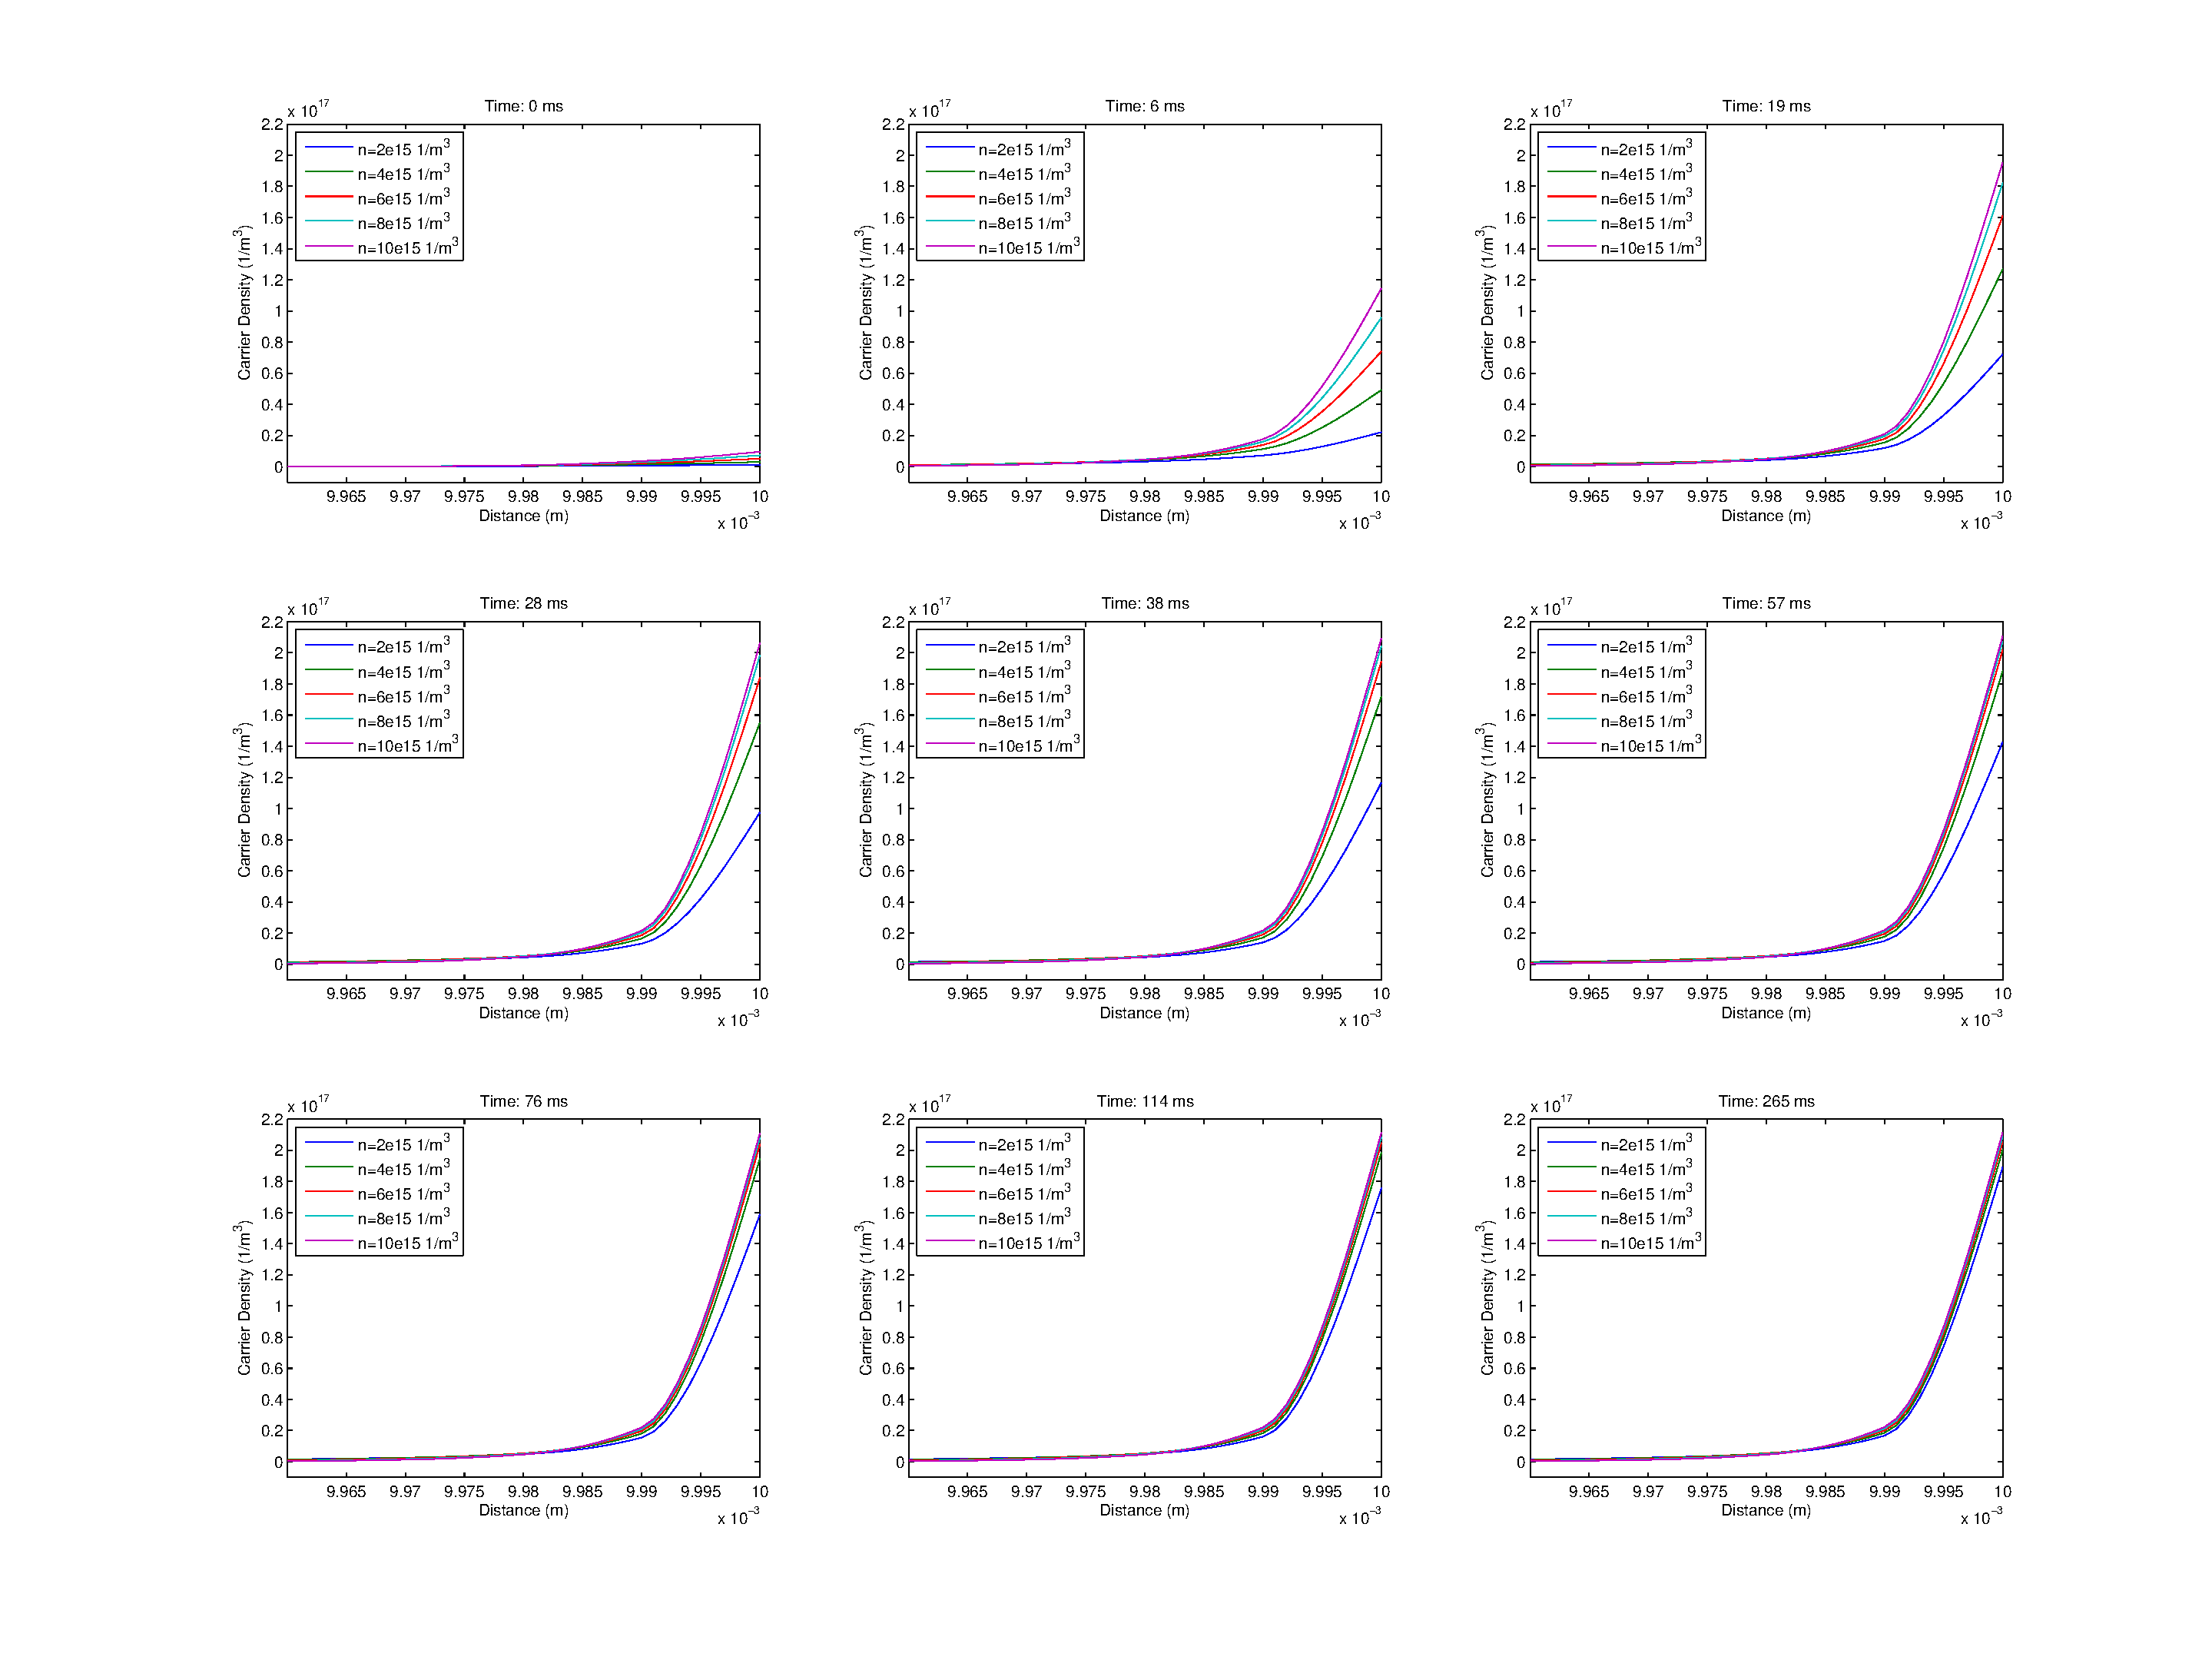
\includegraphics[scale=0.40]{Ex1NetQ_Time}
\caption{Normalized net charge density distribution in electrolyte over time} 
\label{ElectrolyteQzoom}
\end{figure}
\end{landscape}

\begin{landscape}
\begin{figure}[!htp]
\centering
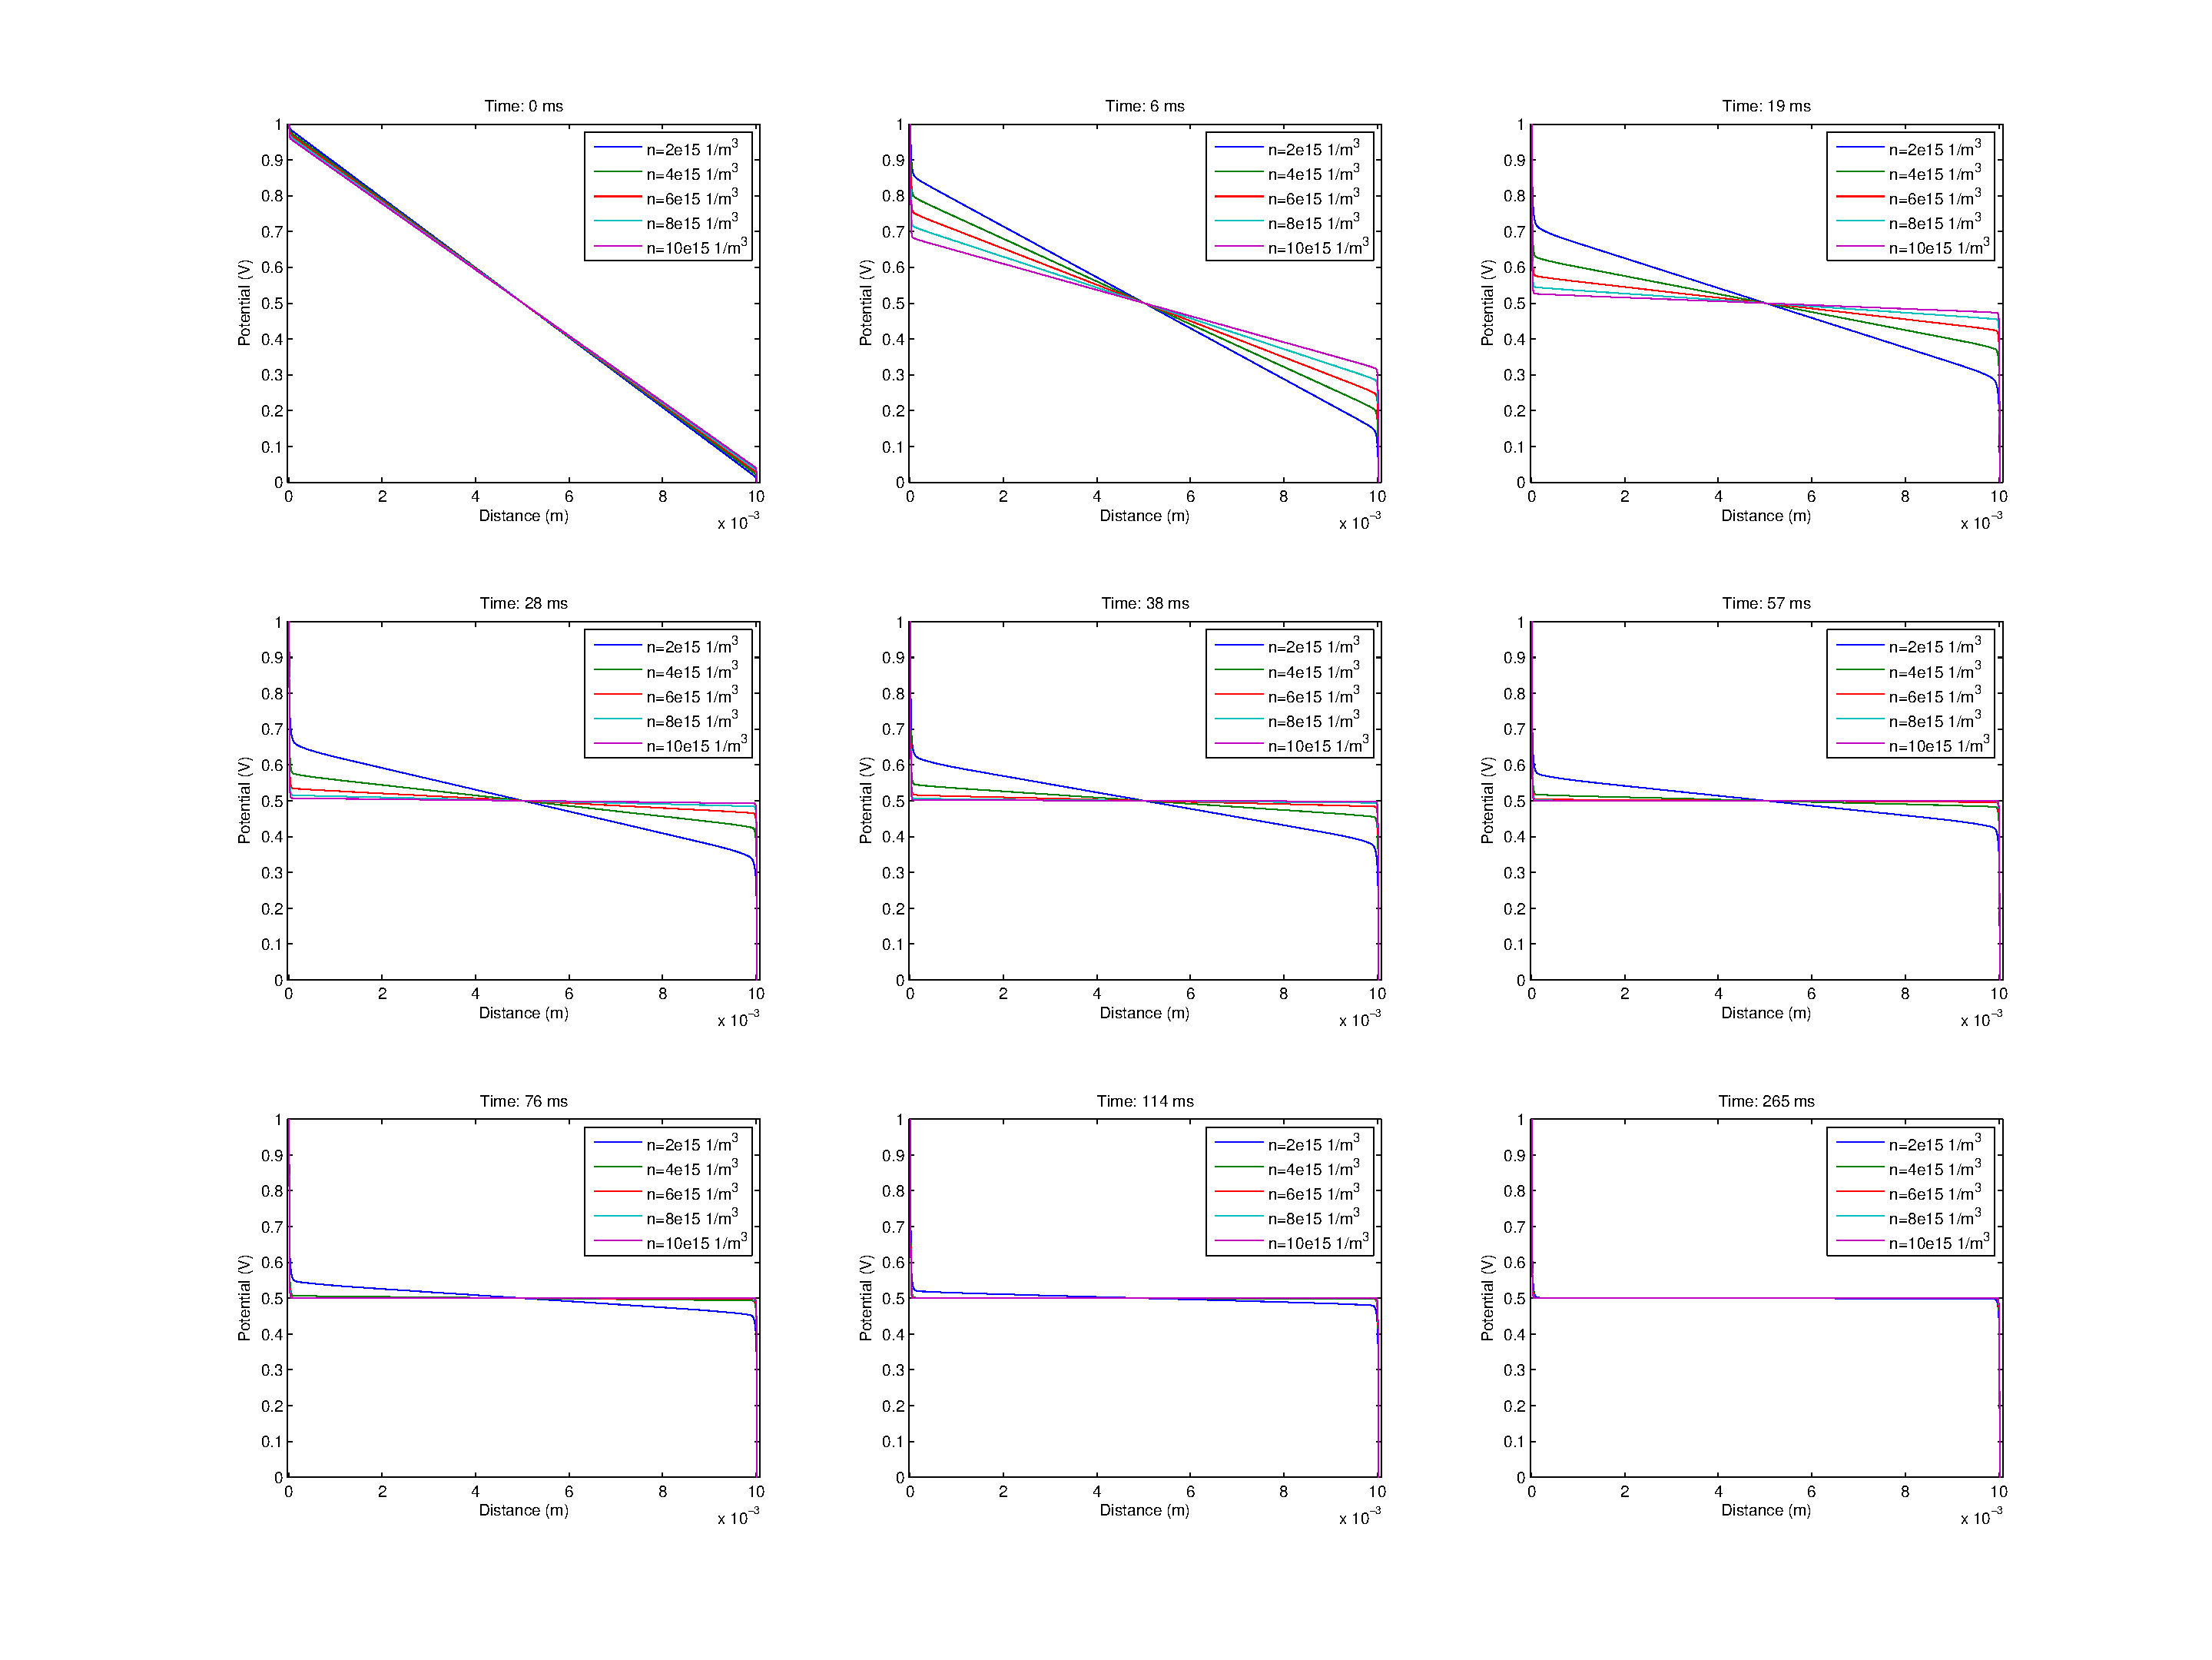
\includegraphics[scale=0.40]{Ex1V_Time}
\caption{Potential distribution in electrolyte over time} 
\label{ElectrolyteV}
\end{figure}
\end{landscape}

 
\begin{landscape}
\begin{figure}[!htp]
\centering
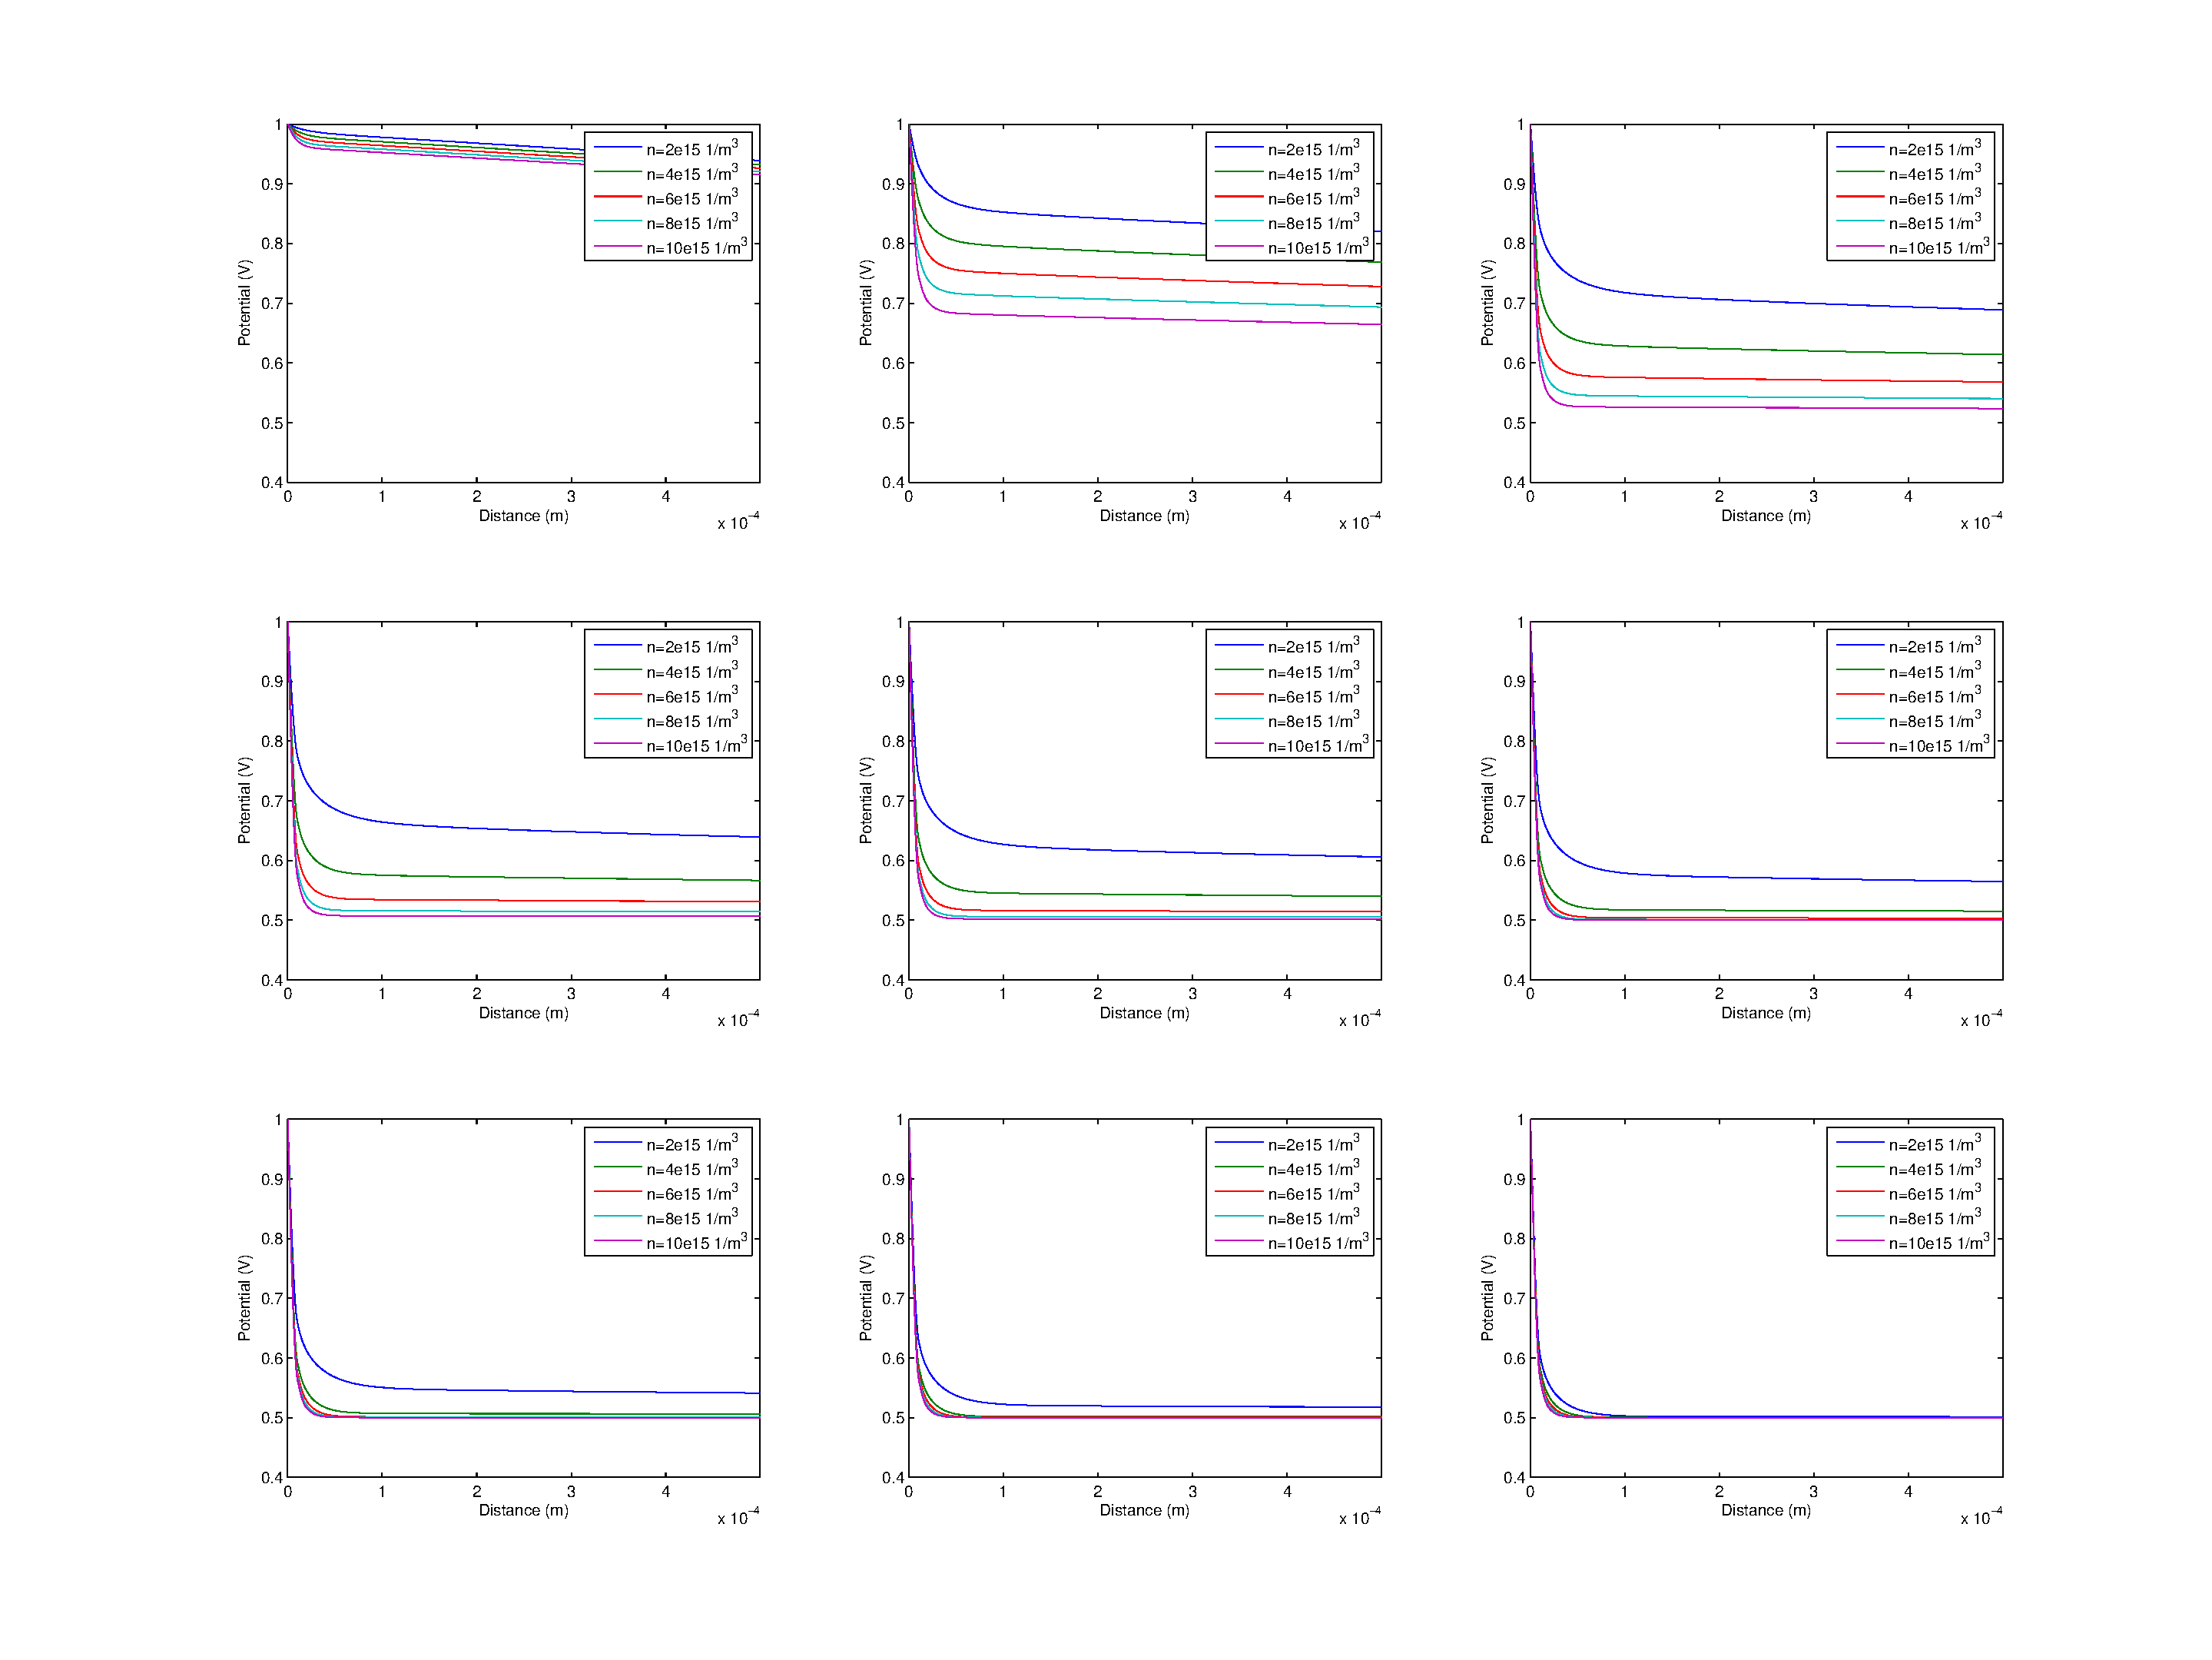
\includegraphics[scale=0.40]{Ex1V_Time2}
\caption{Potential distribution on the left wall of the electrolyte over time} 
\label{ElectrolyteV2}
\end{figure}
\end{landscape}

\clearpage
\subsection{1-D Horizontal Memristor (Cross Section 2)}

Cross section 2 from figure \ref{MemStc} has the most crucial elements of the memristor but its simulation in 1-D is not as straight forward as the simulation of the electrolyte. Horizontal cross section through the PEDOT does not include the vertical movement of lithium. Without this effect PEDOT is just a regular conductor with a uniform current density. In order to overcome this problem a generation/recombination term for lithium ions, calculated at every time step, was added to capture the vertical movement in addition to regular drift diffusion equations which represents the horizontal movement. This generation/recombination term can be represented as a current source with a resistor connected to every node (figure \ref{MemStc15}). 

The lithium source has two different terms, one for drift and another one for diffusion. It was assumed that the concentration of lithium was always constant in the electrolyte. This way the vertical diffusion current density can be calculated using the difference between the lithium density in PEDOT and electrolyte. For the diffusion term an electric field has to be estimated between the PEDOT and the electrolyte. First the potential of the electrolyte was assumed to be half of the net applied potential. Then an electric field is calculated using the electrolyte and the potential of the PEDOT at different positions.
  
\begin{figure}[!htp]
\centering
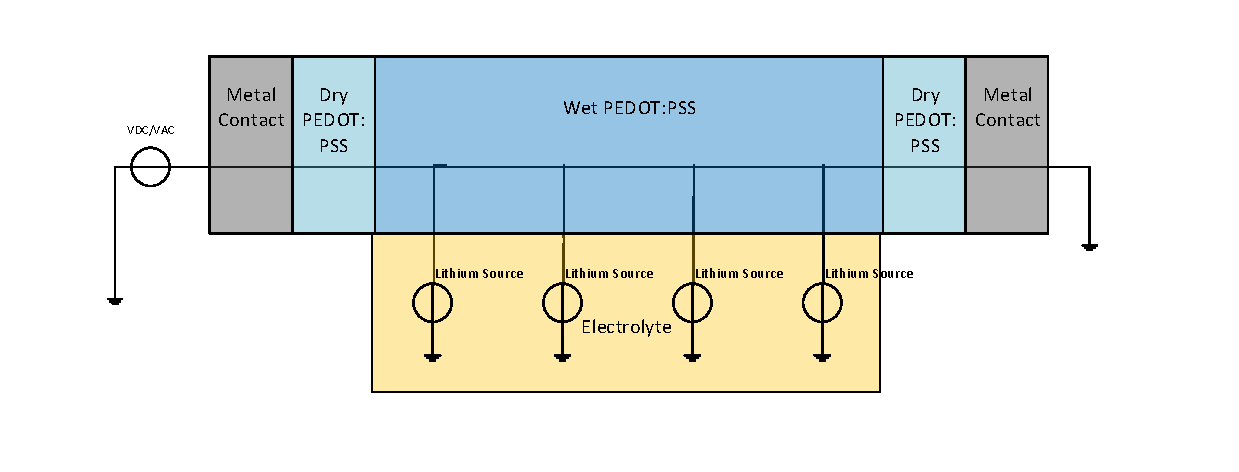
\includegraphics[scale=0.74]{1DMem}
\caption{1.5-D Memristor Structure} 
\label{MemStc15}
\end{figure}


\begin{landscape}
\begin{figure}[!htp]
\centering
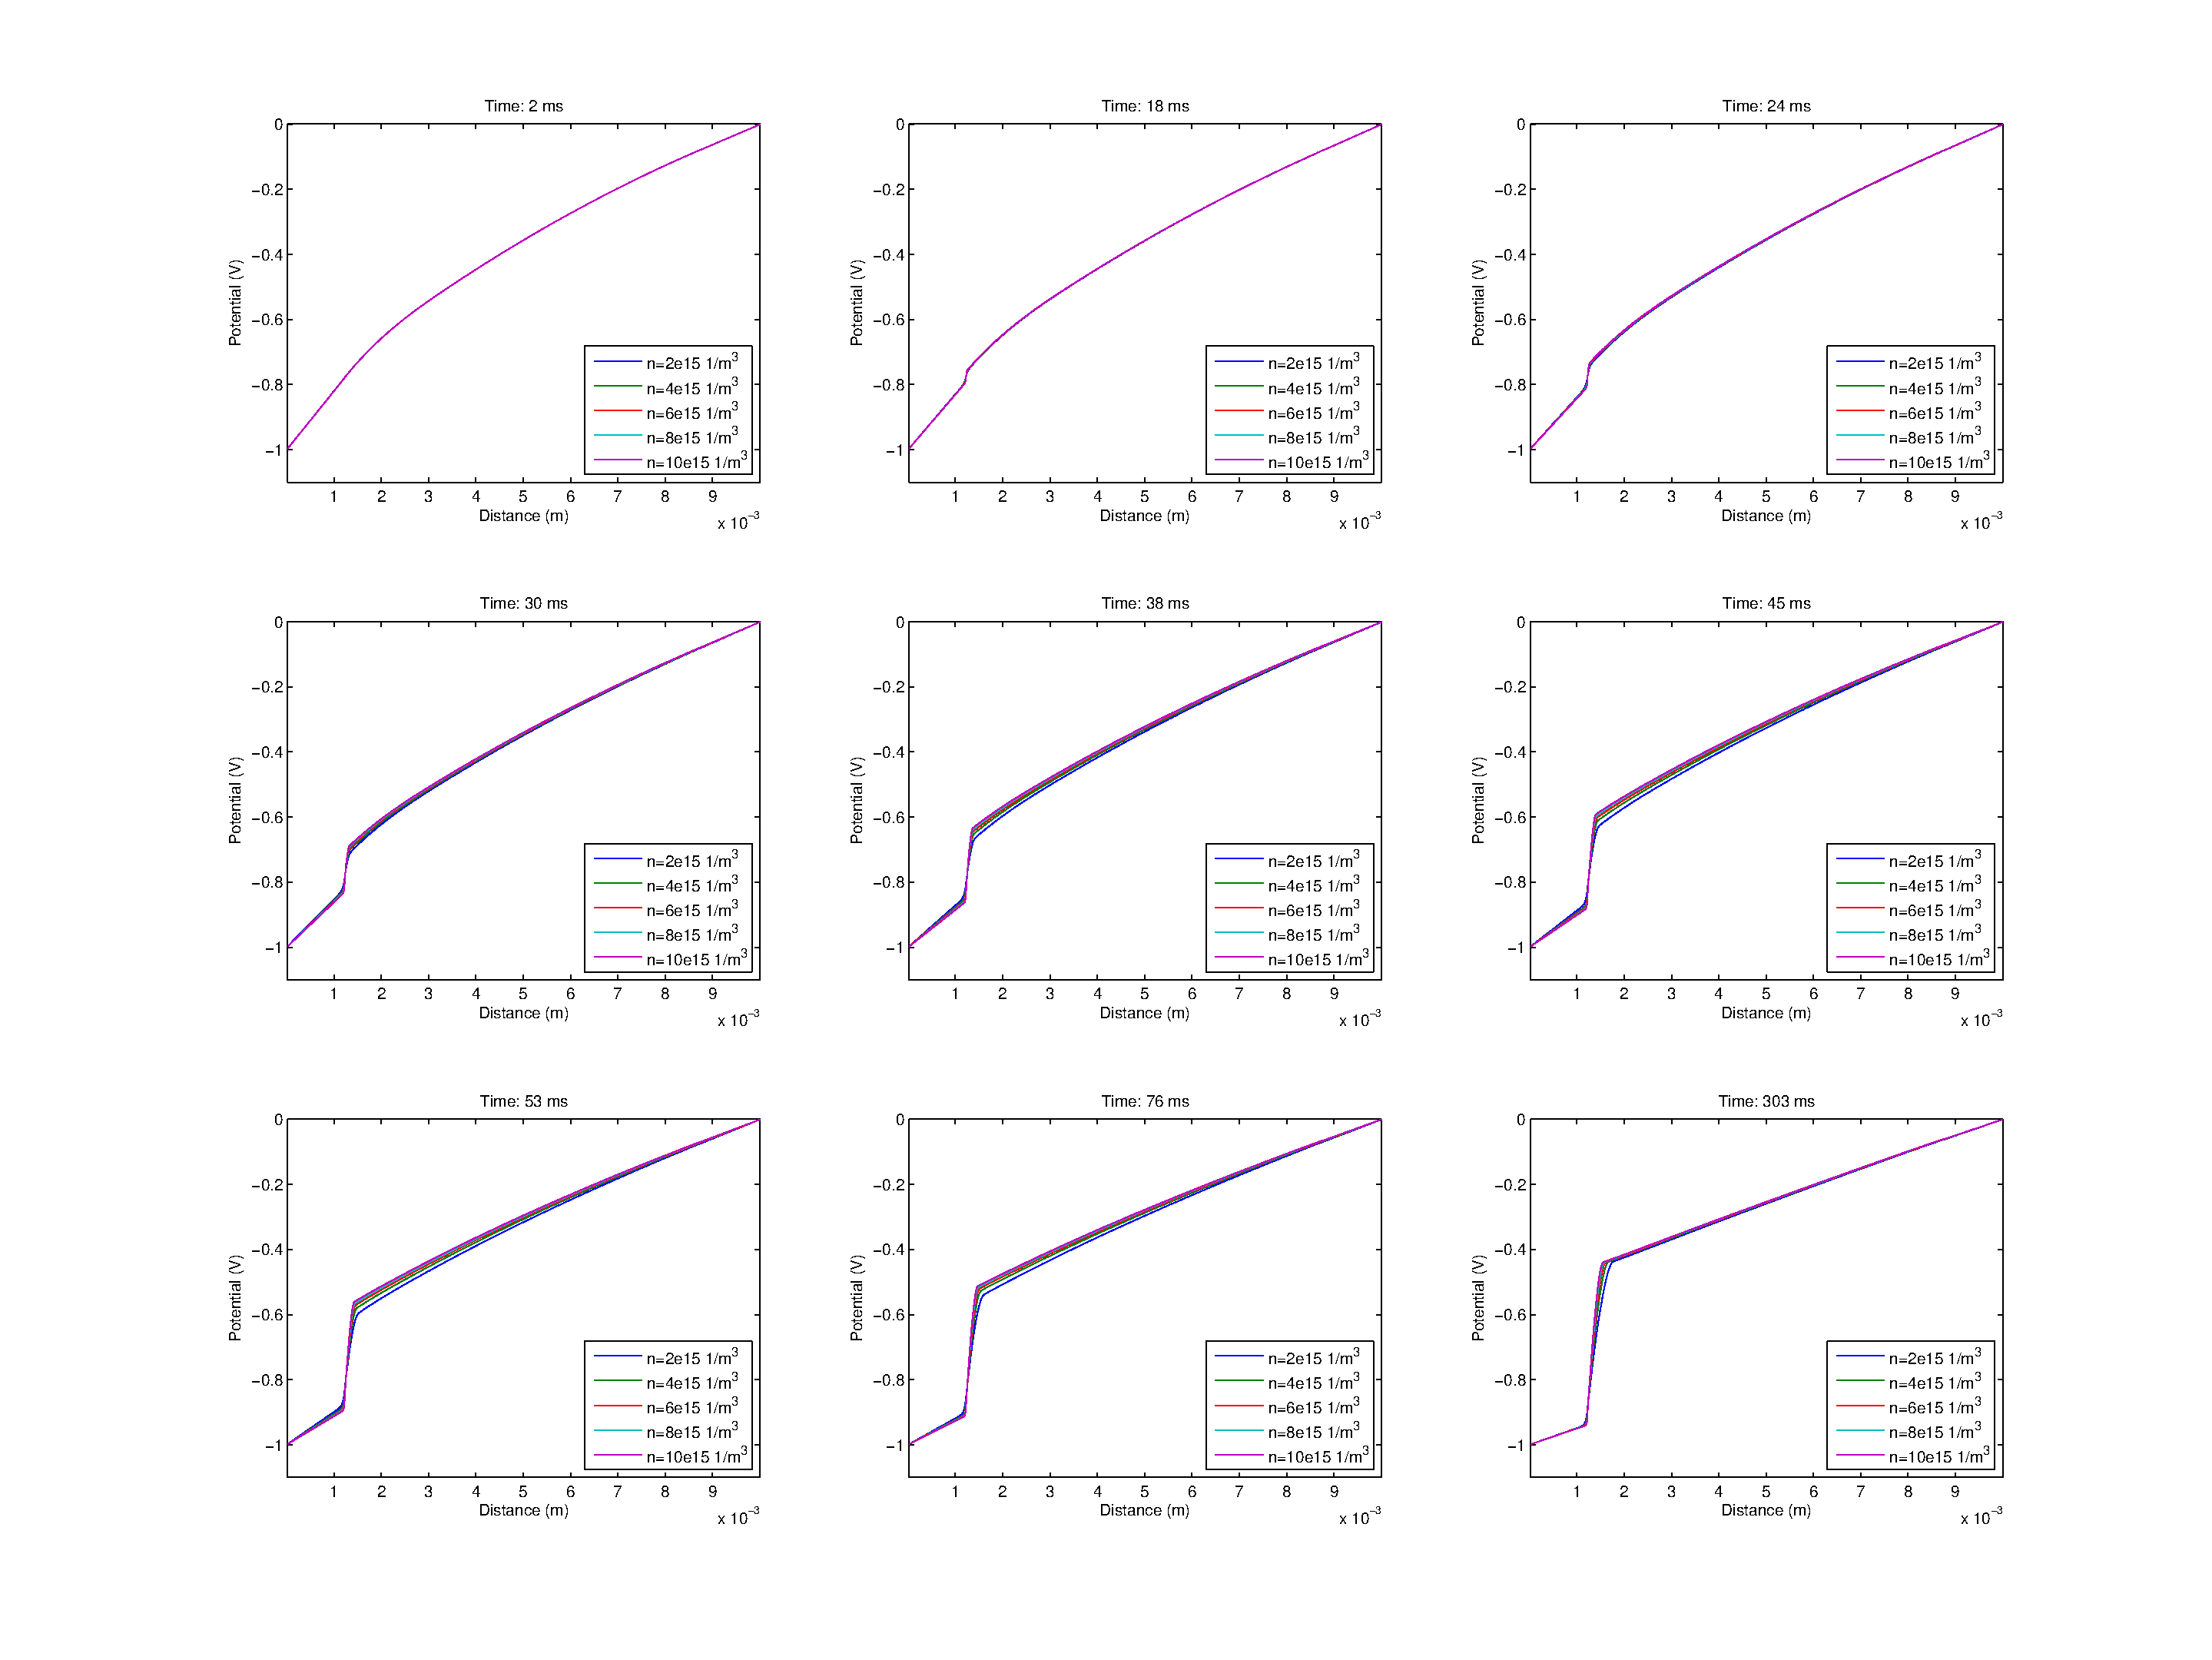
\includegraphics[scale=0.40]{Ex5V_Time1}
\caption{1-D Memristor potential distribution over time} 
\label{}
\end{figure}
\end{landscape}


\begin{landscape}
\begin{figure}[!htp]
\centering
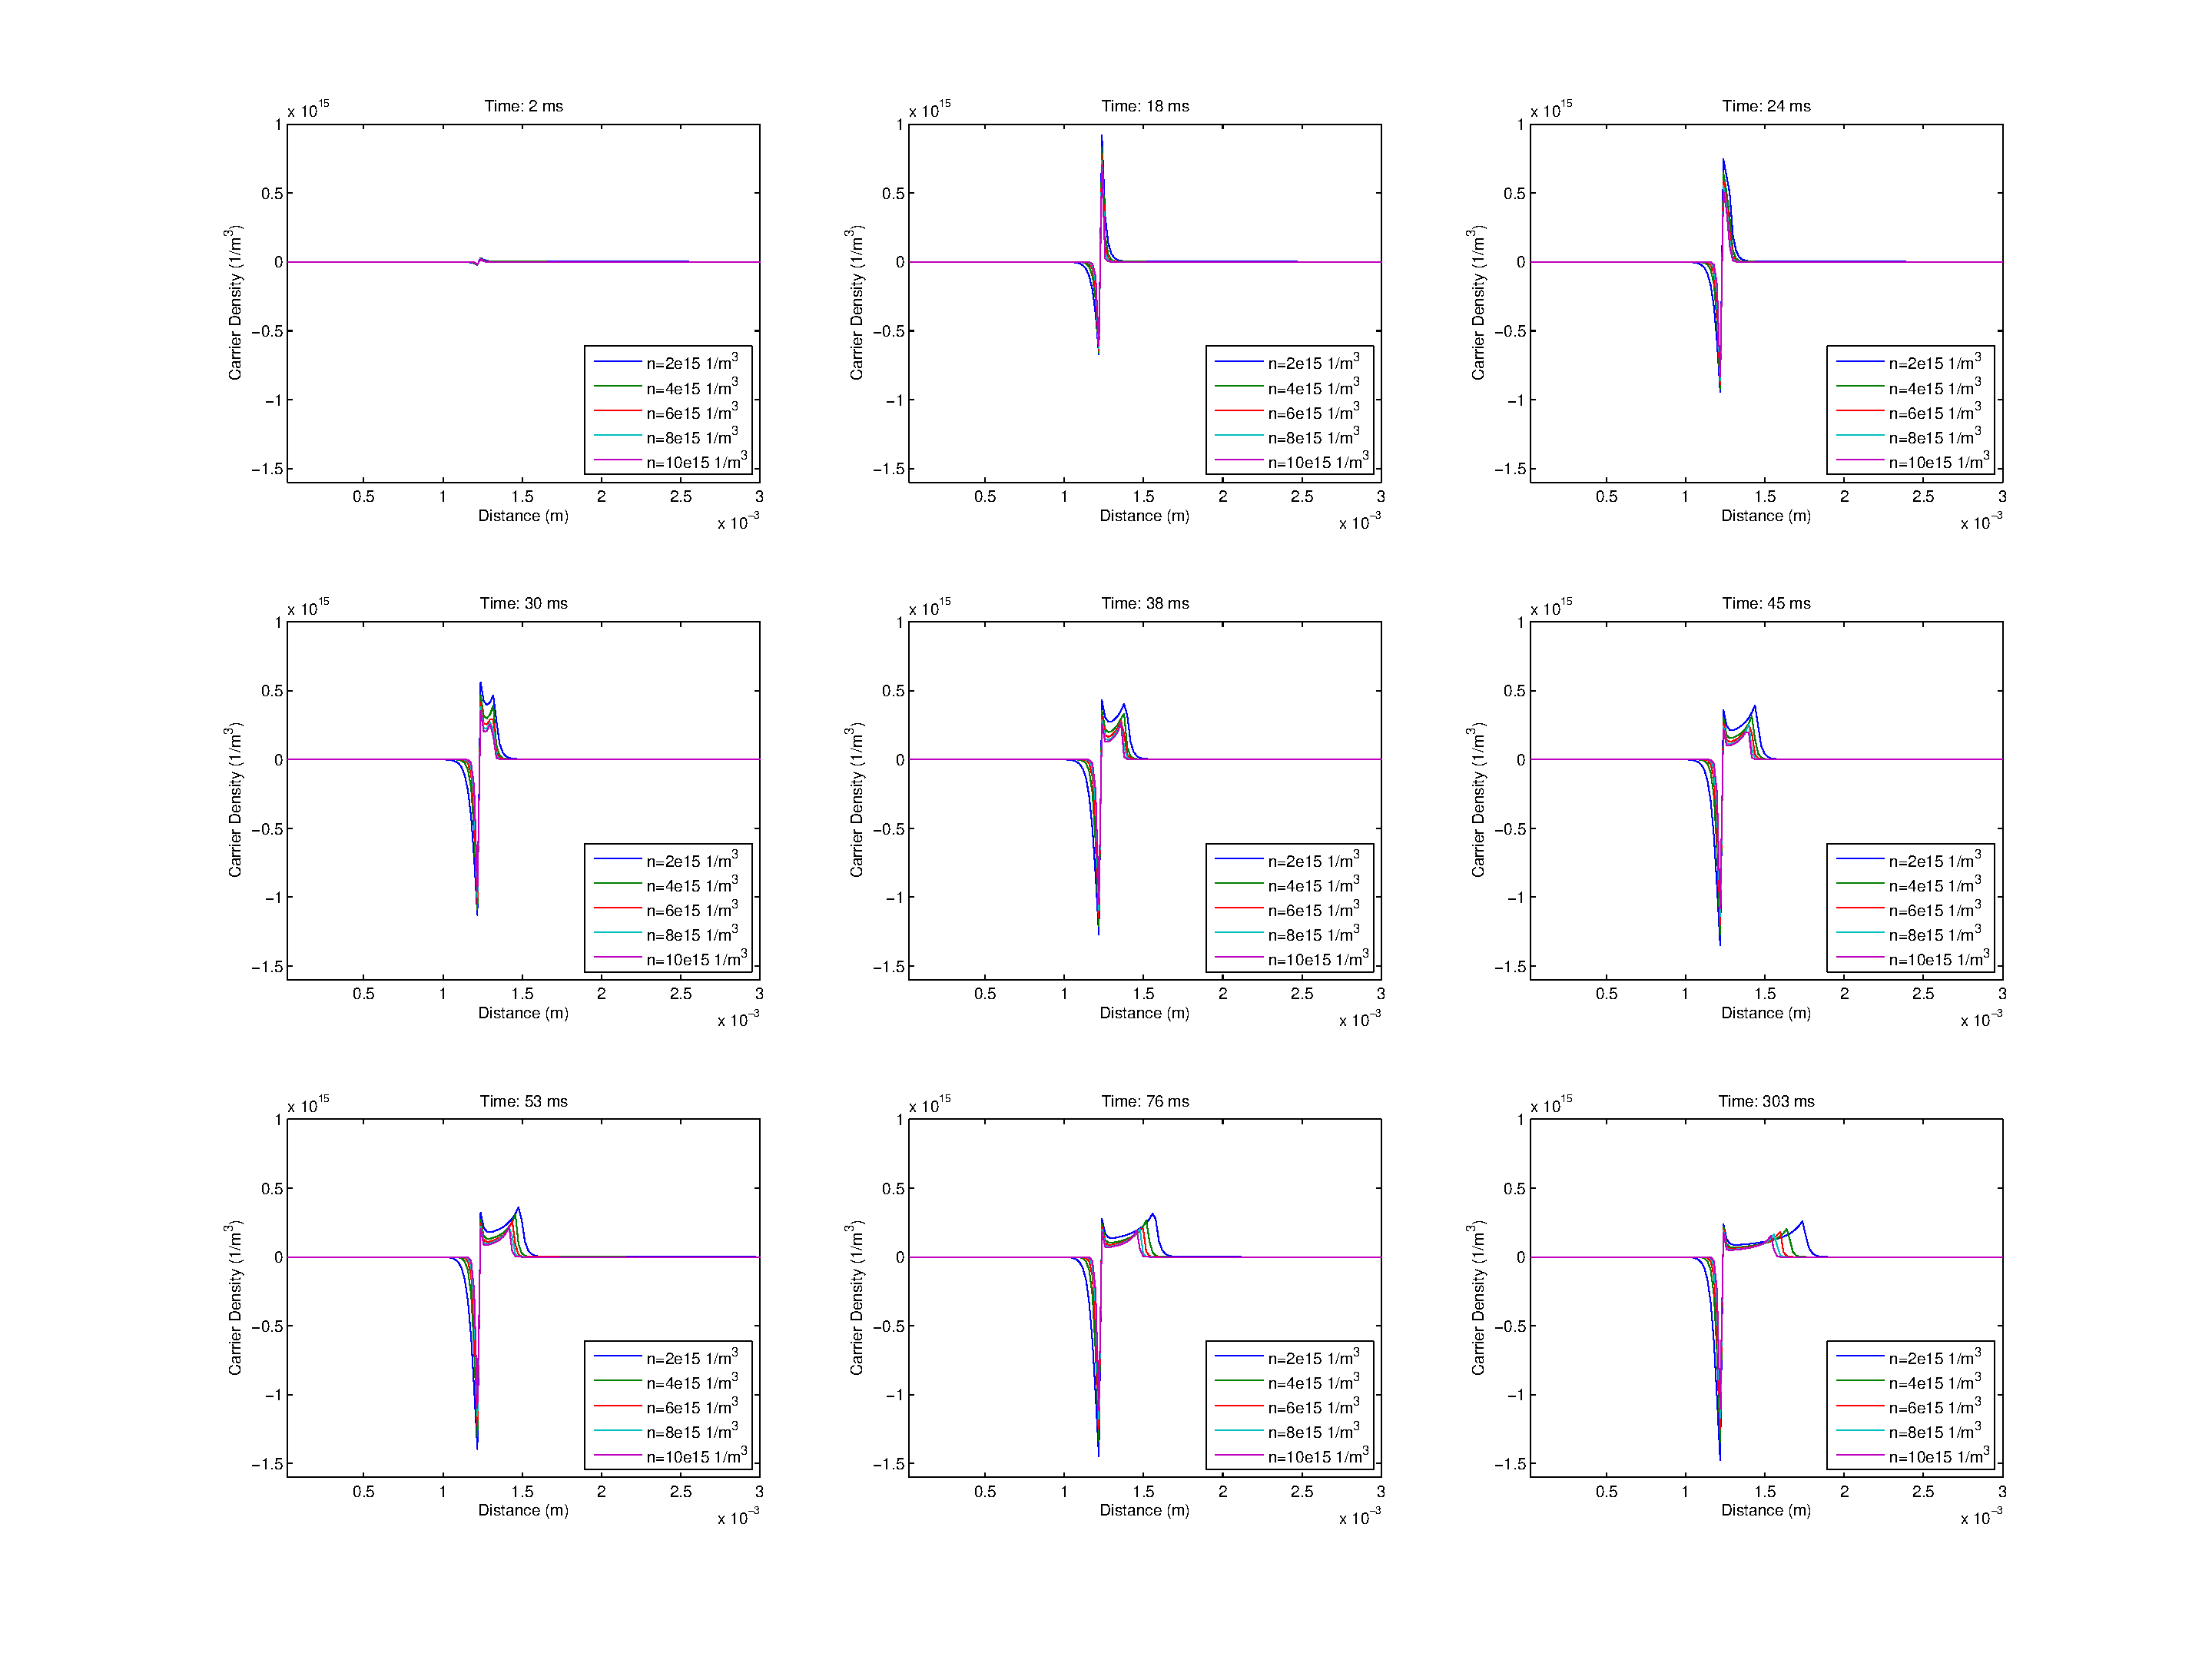
\includegraphics[scale=0.40]{Ex5NetQ_Time1}
\caption{Normalized net charge density distribution over time} 
\label{}
\end{figure}
\end{landscape}


\begin{landscape}
\begin{figure}[!htp]
\centering
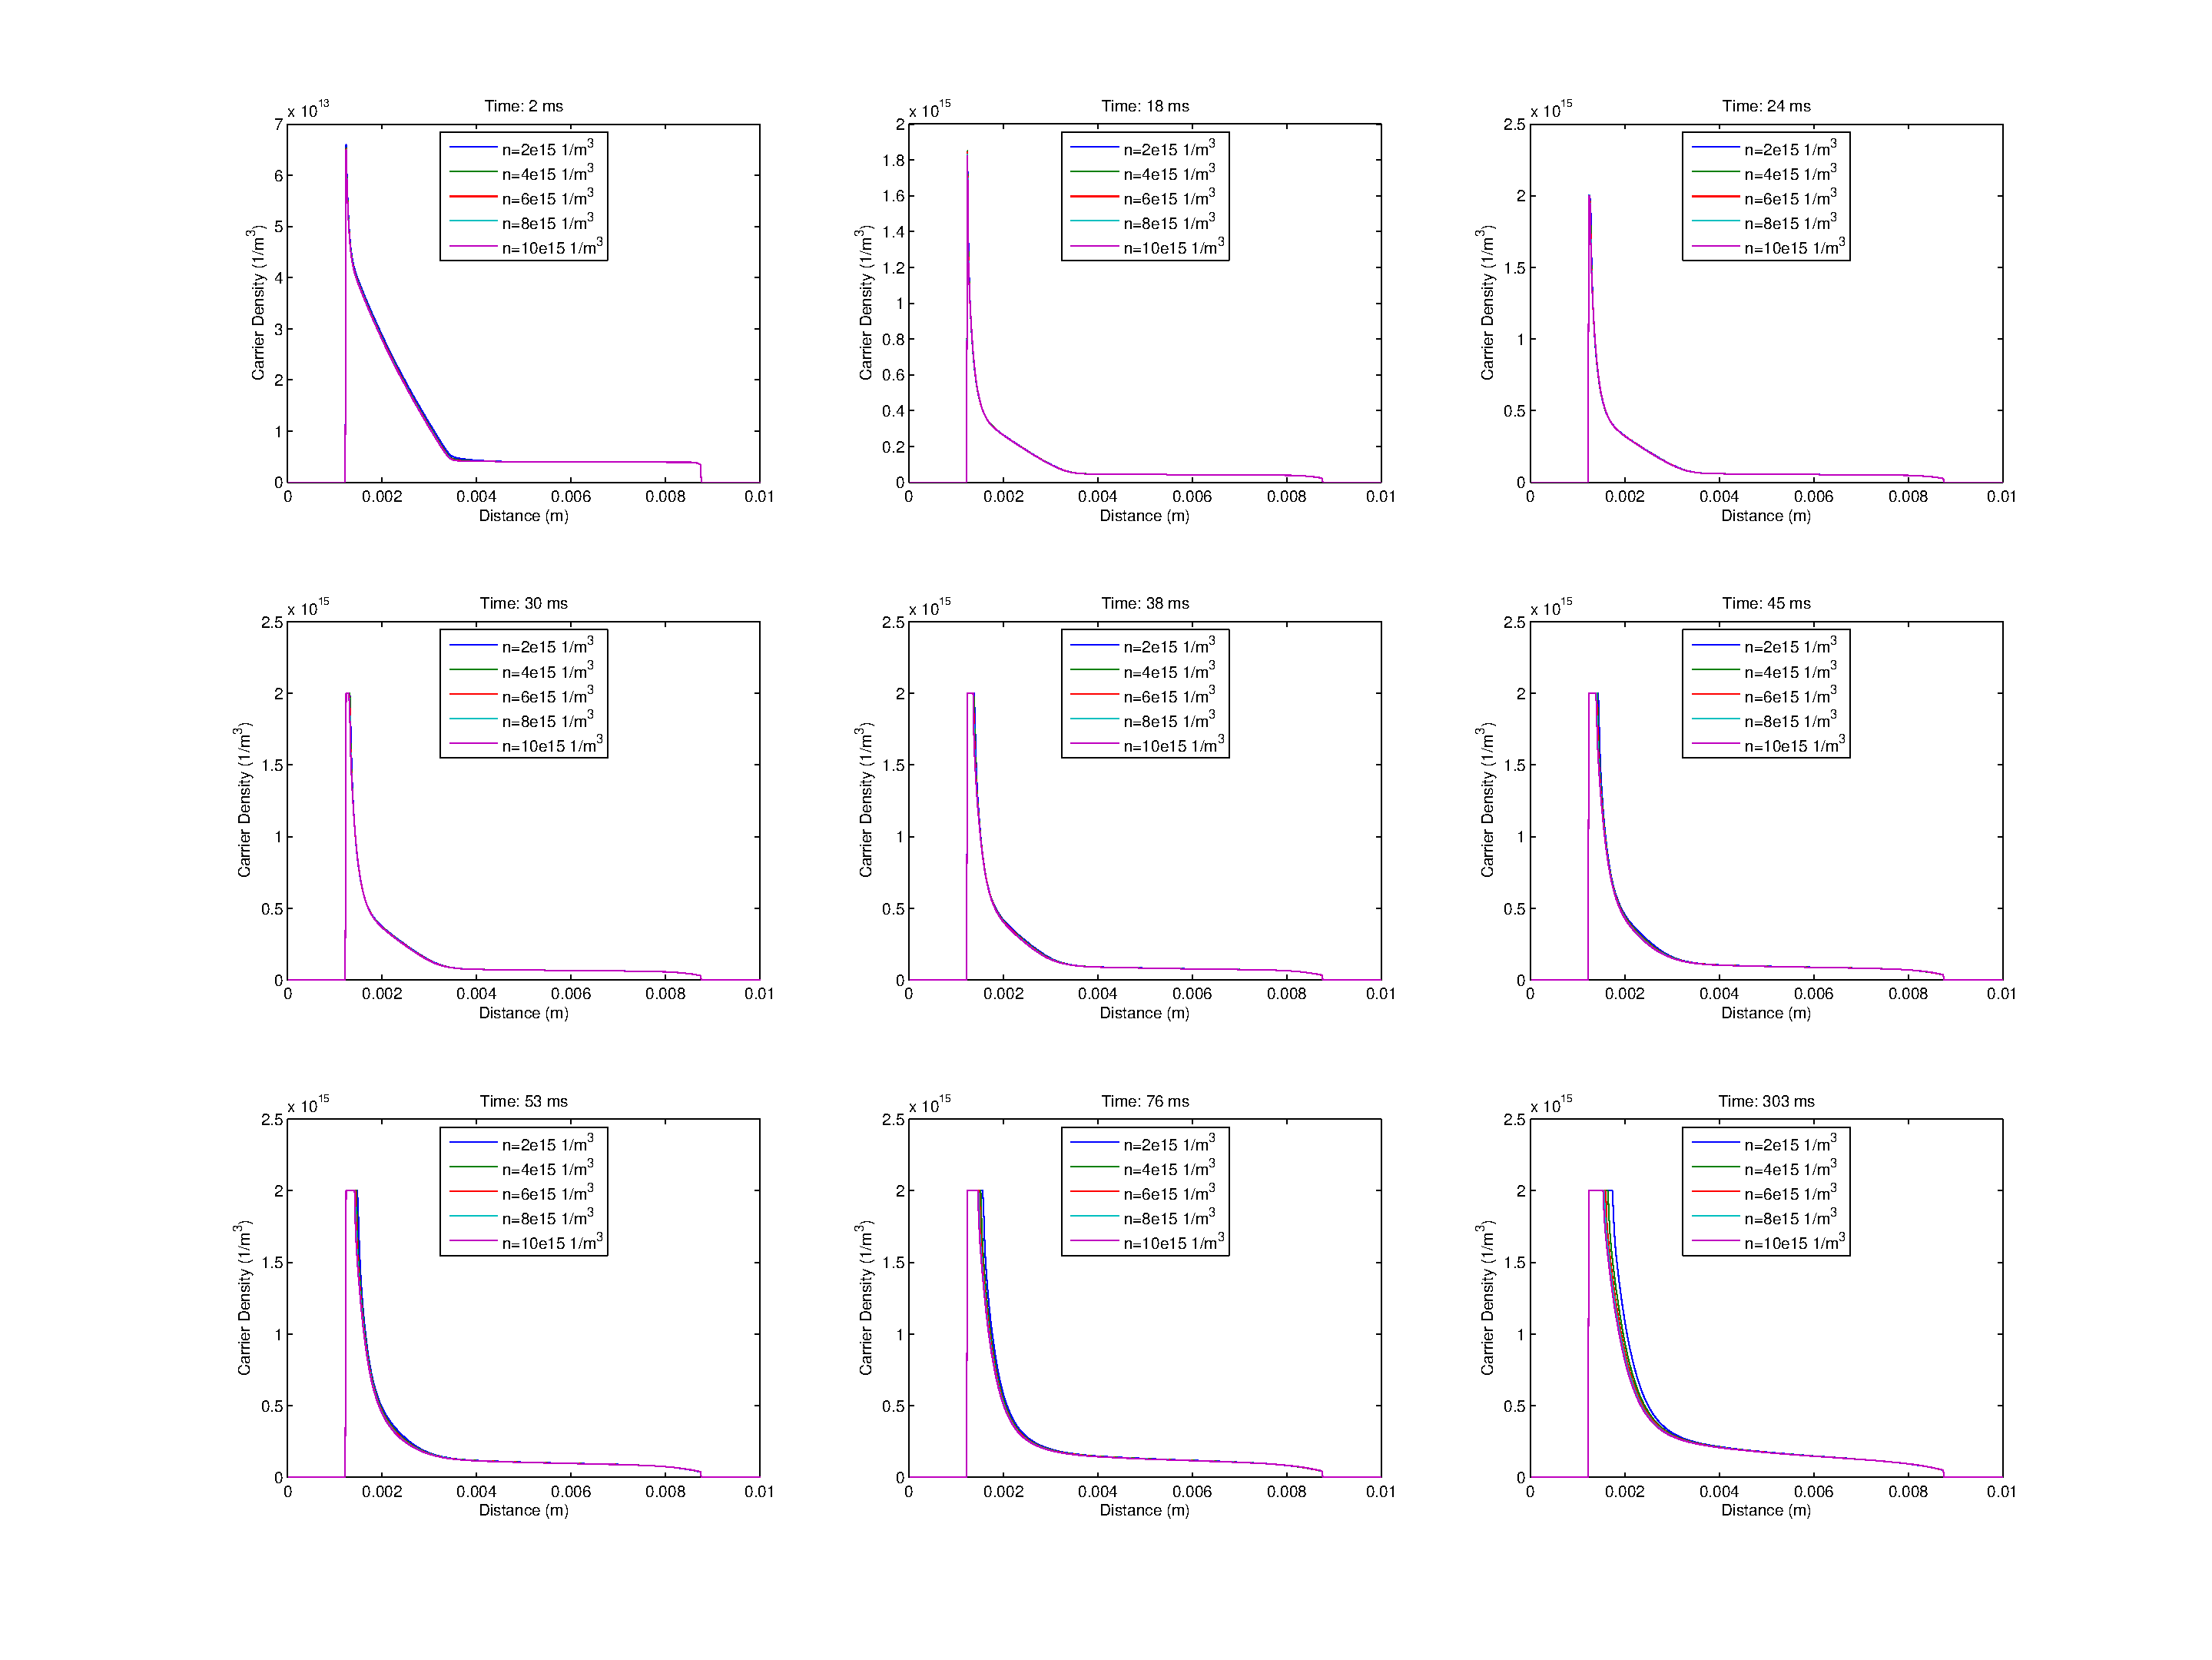
\includegraphics[scale=0.40]{Ex5Np_Time1}
\caption{Normalized lithium density distribution over time} 
\label{}
\end{figure}
\end{landscape}


\begin{landscape}
\begin{figure}[!htp]
\centering
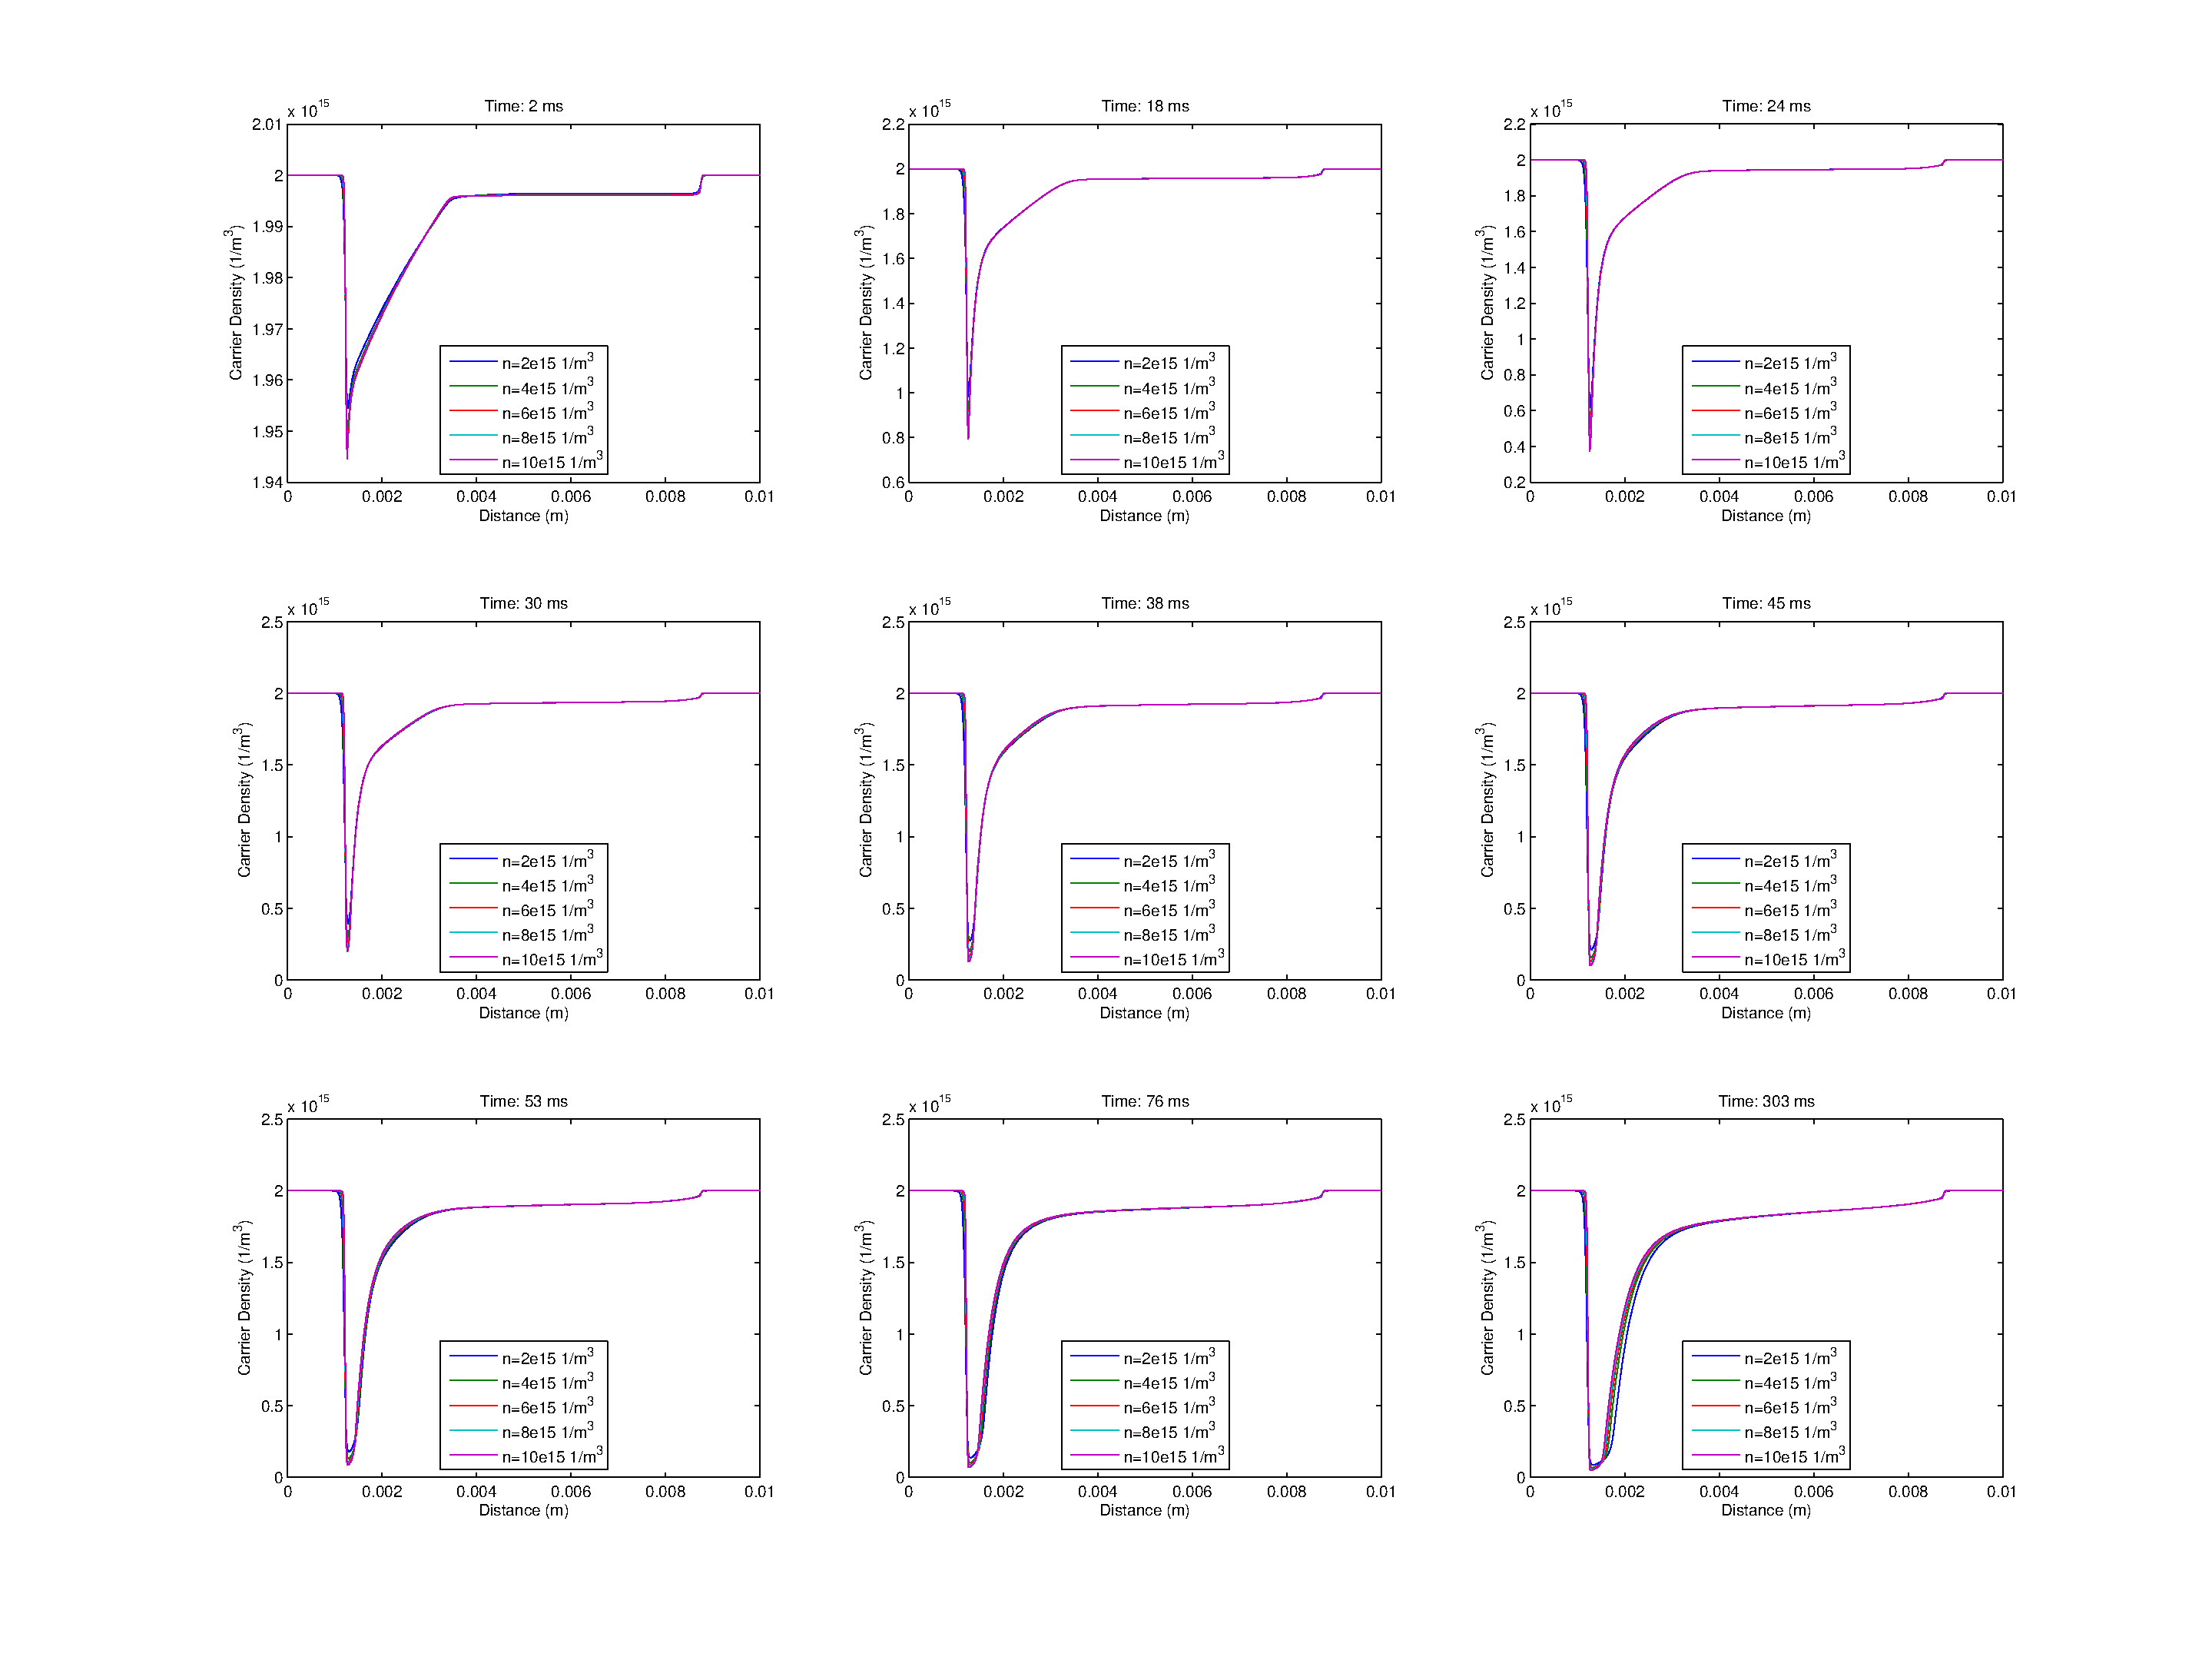
\includegraphics[scale=0.40]{Ex5p_Time1}
\caption{Normalized hole density distribution over time} 
\label{}
\end{figure}
\end{landscape}

\begin{landscape}
\begin{figure}[!htp]
\centering
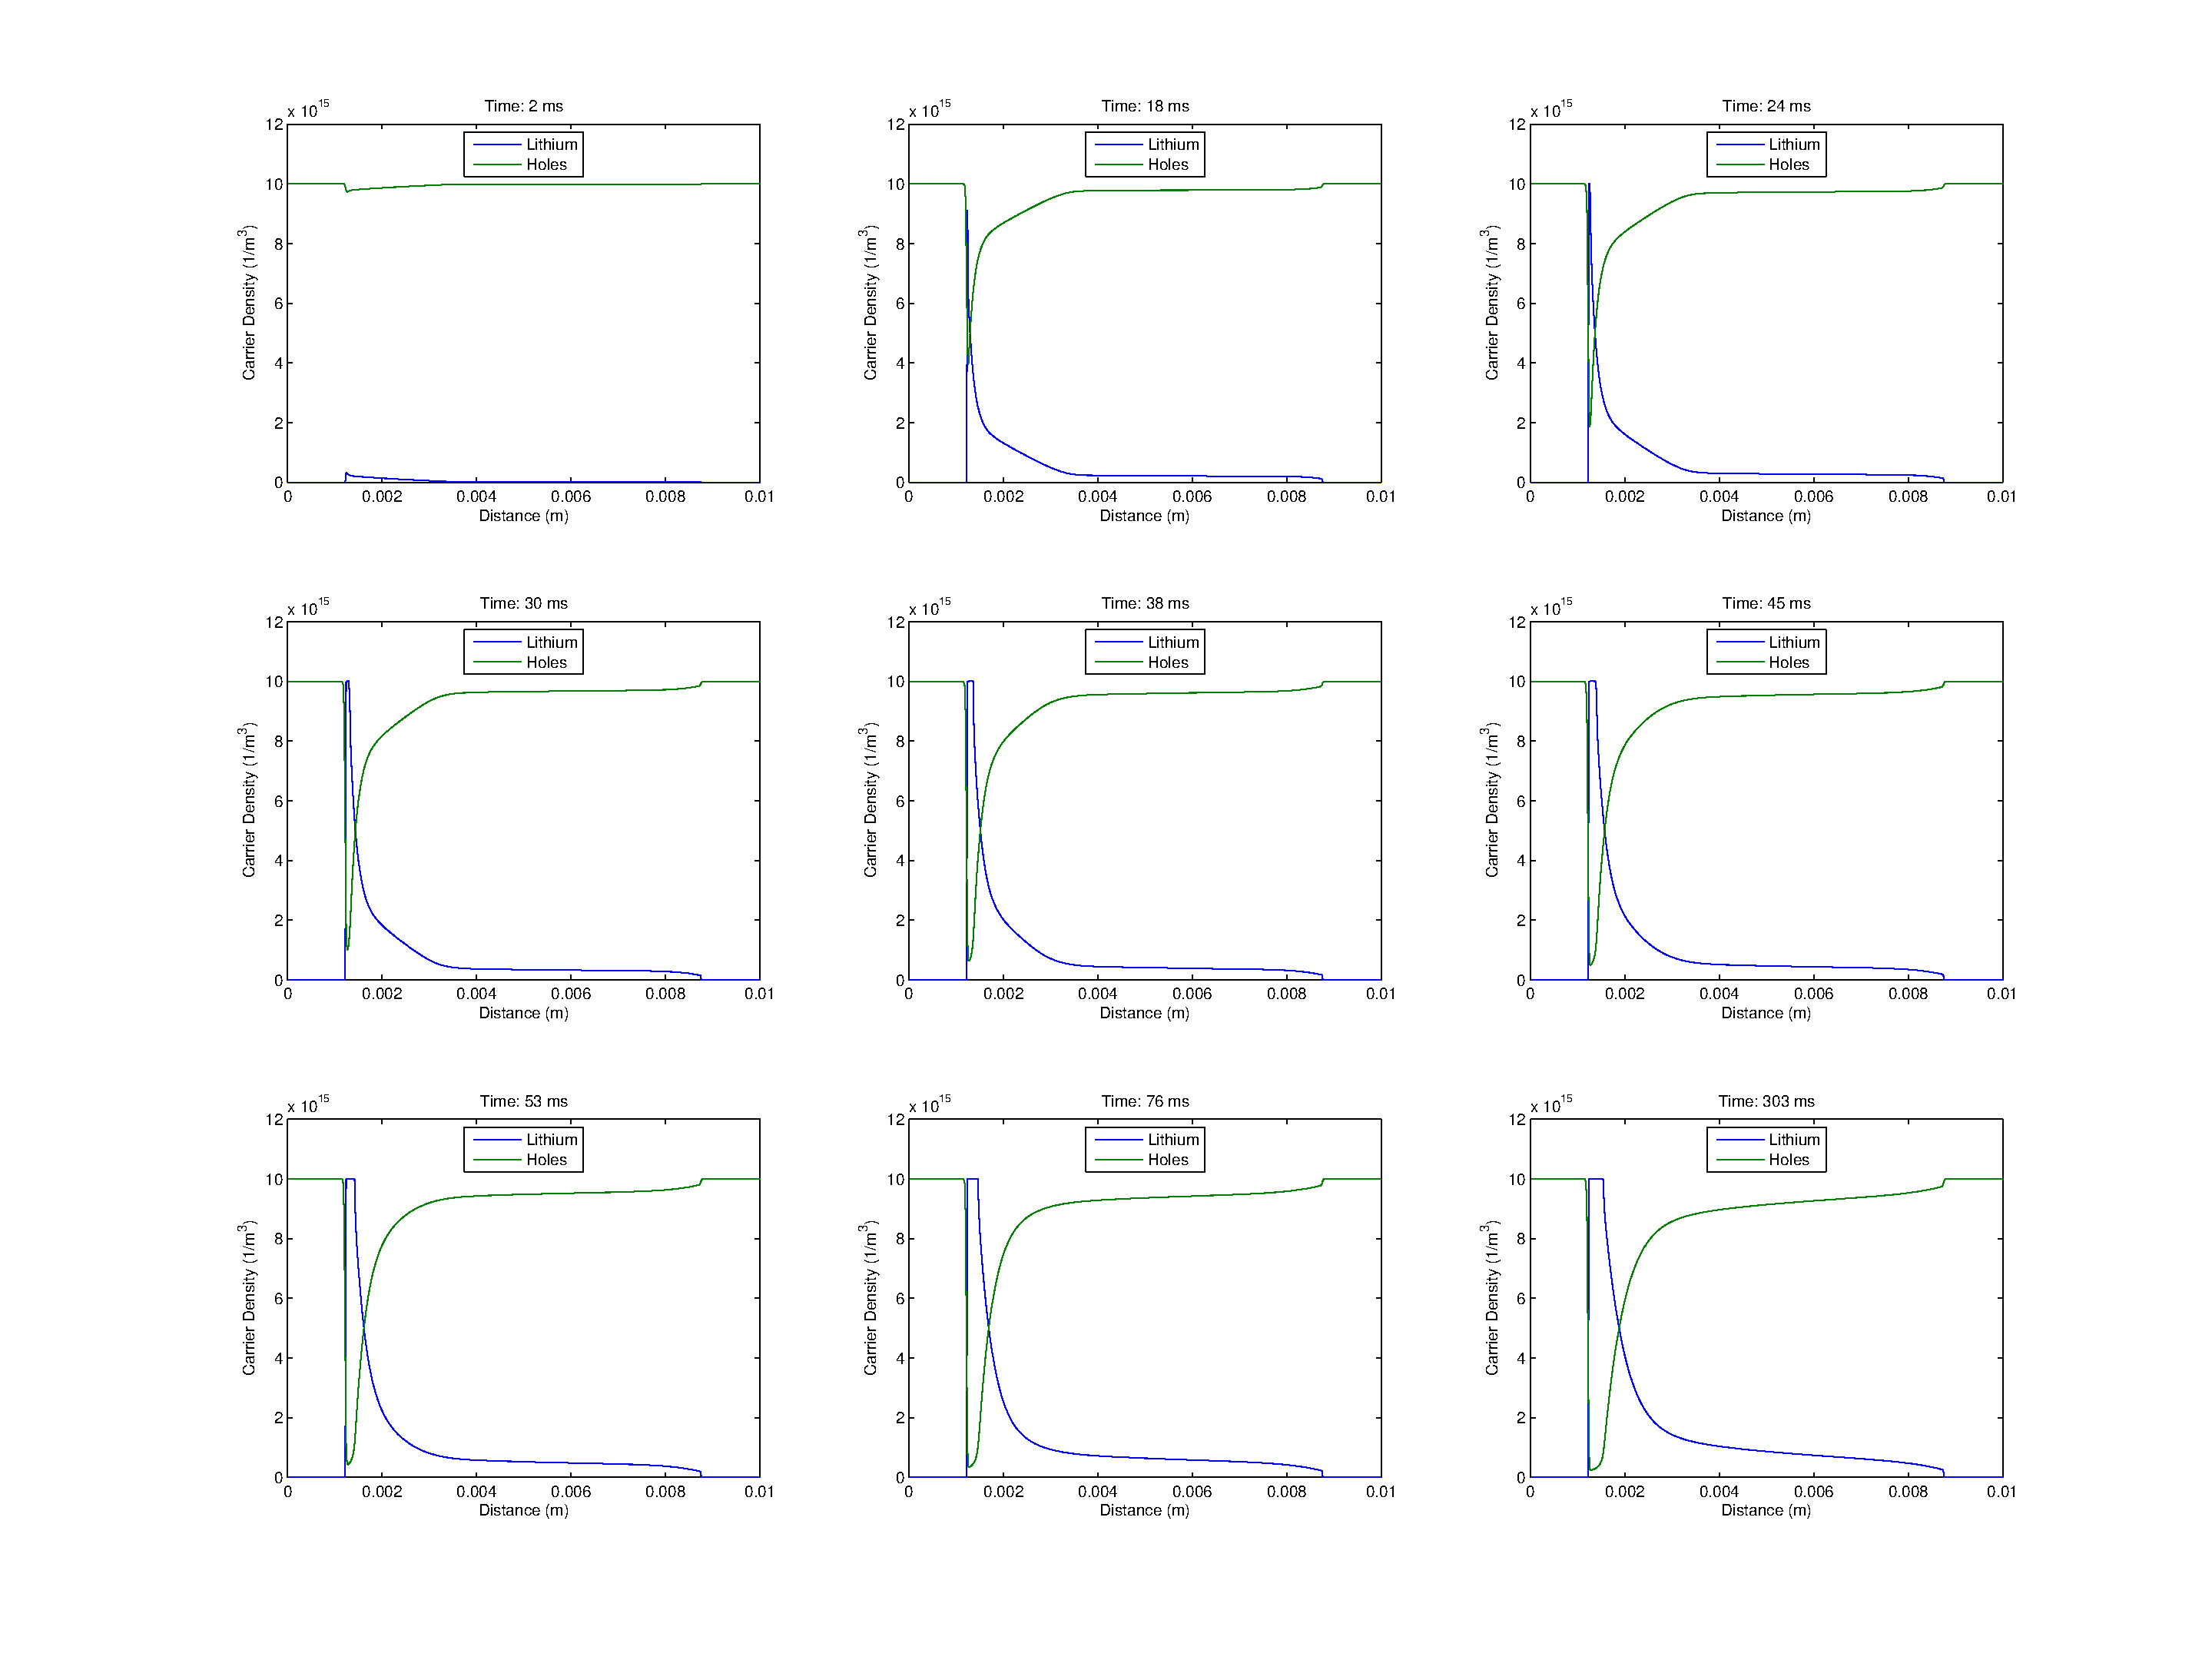
\includegraphics[scale=0.40]{Ex5pNp_Time1}
\caption{Lithium and hole density distribution over time} 
\label{}
\end{figure}
\end{landscape}



\begin{figure}[!htp]
\centering
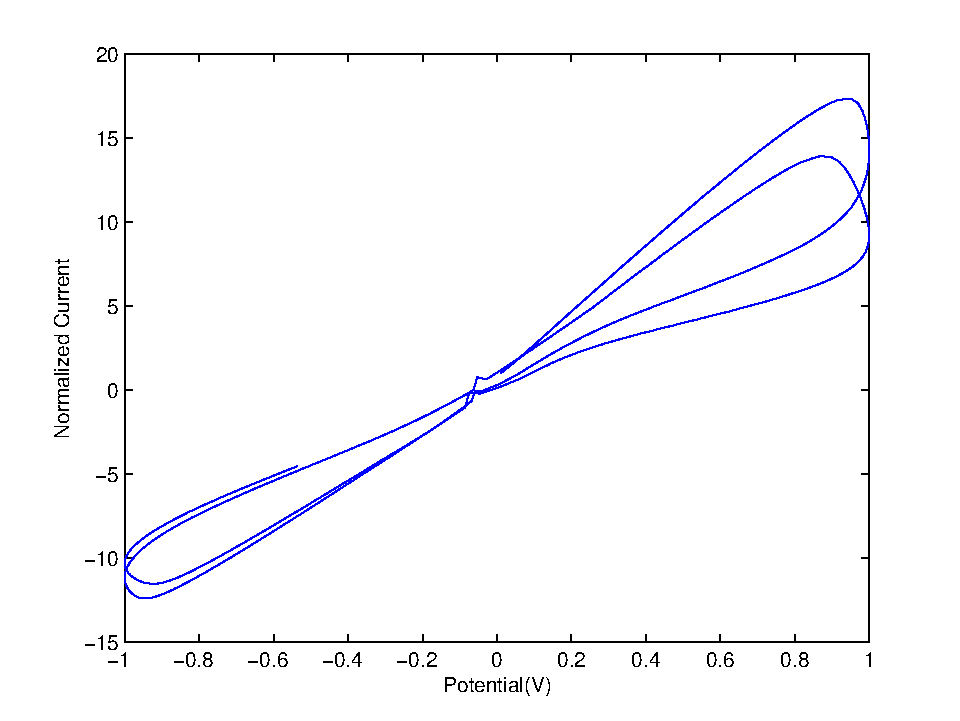
\includegraphics[scale=0.60]{Ex5Bowtie}
\caption{Normalized Current vs. potential} 
\label{}
\end{figure}

\begin{figure}[!htp]
\centering
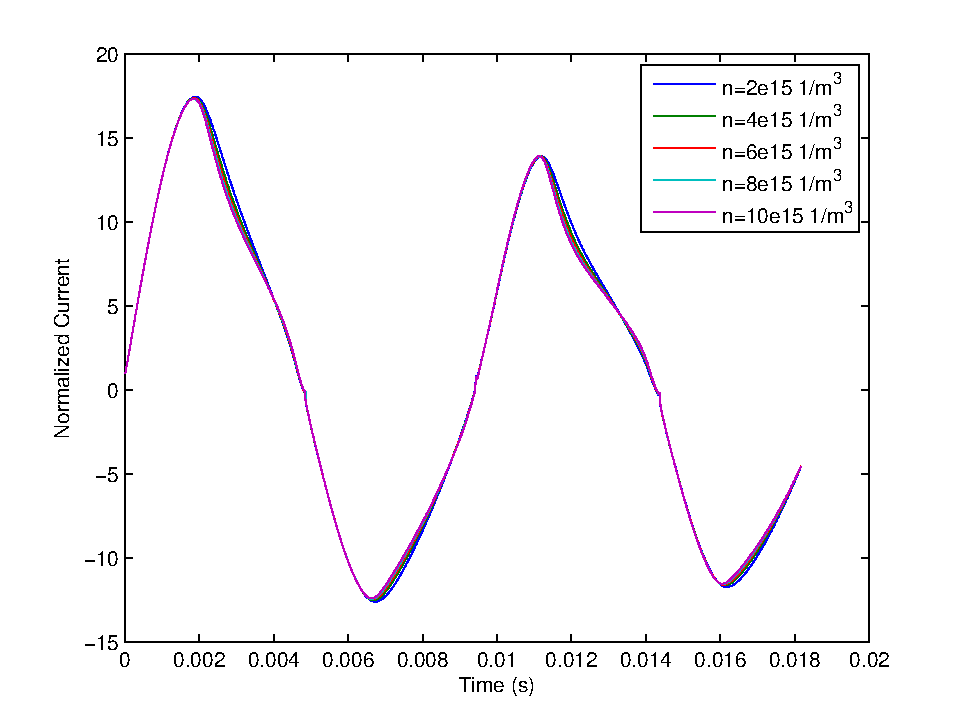
\includegraphics[scale=0.60]{Ex5Current}
\caption{Normalized current over time} 
\label{}
\end{figure}



\clearpage
\subsection{PEDOT:PSS with Notch (Cross Section 2)}


\begin{landscape}
\begin{figure}[!htp]
\centering
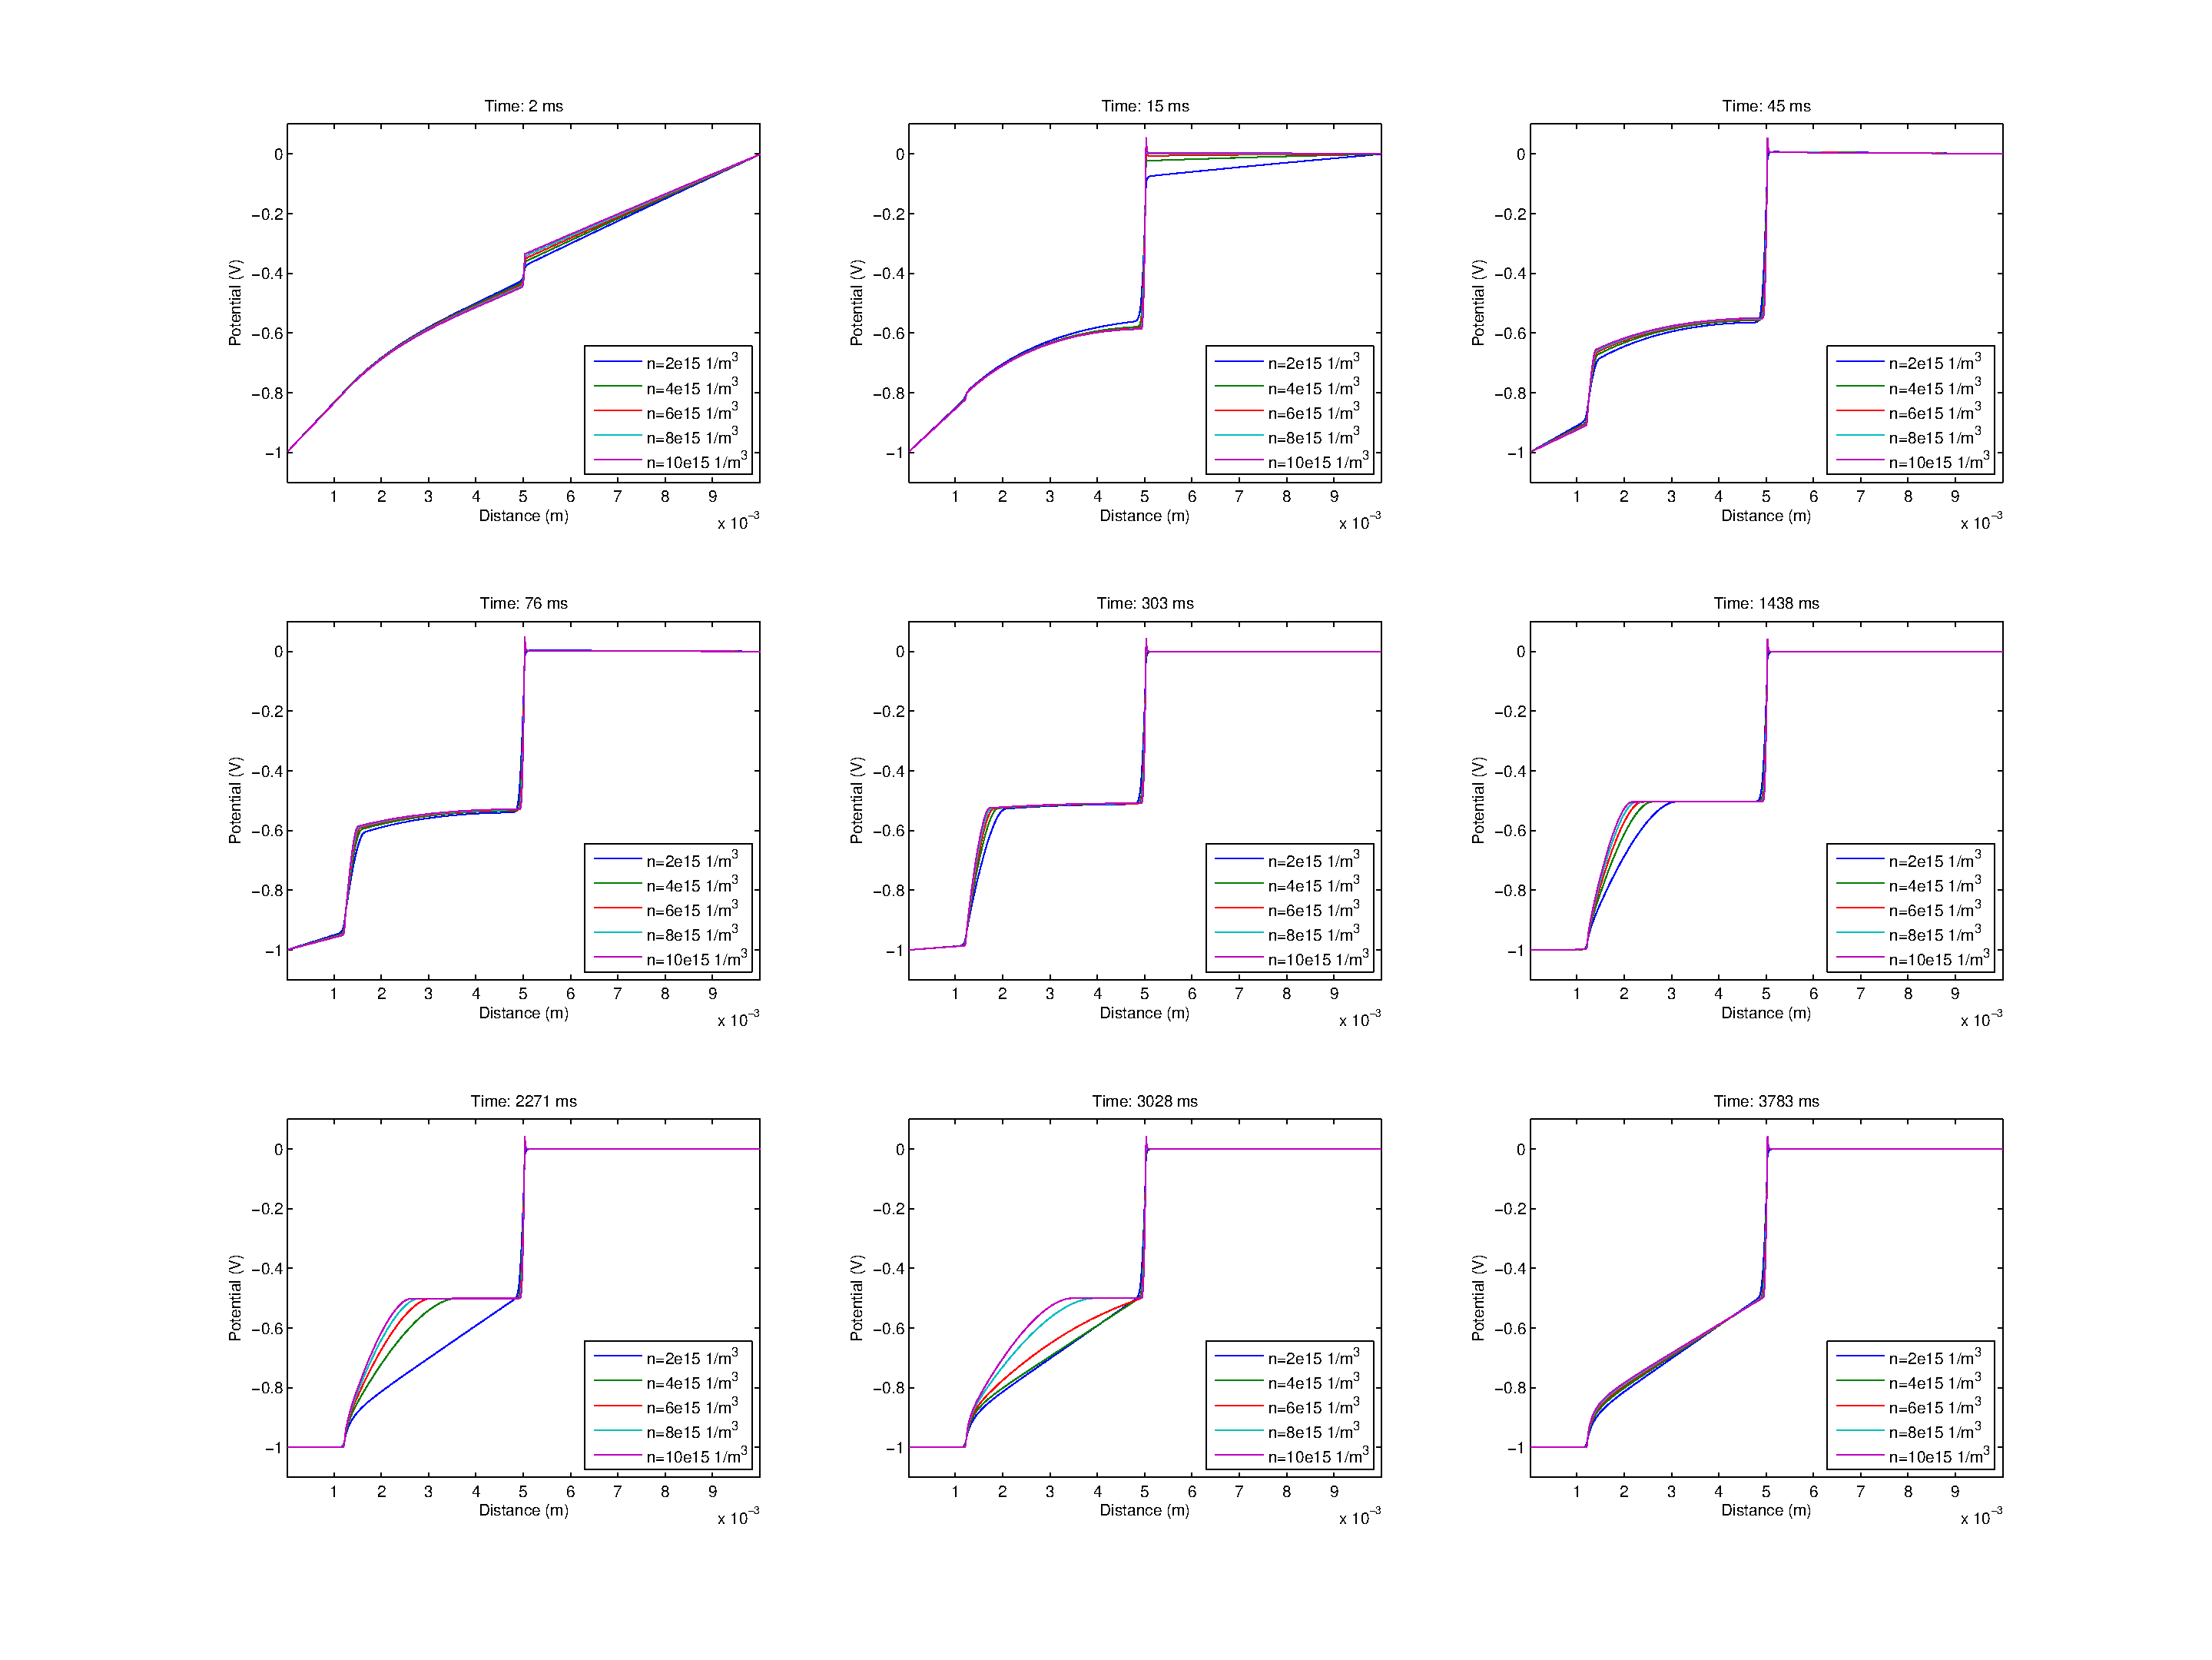
\includegraphics[scale=0.40]{Ex5V_Notch_Time1}
\caption{Notched memristor potential distribution over time} 
\label{}
\end{figure}
\end{landscape}



\begin{landscape}
\begin{figure}[!htp]
\centering
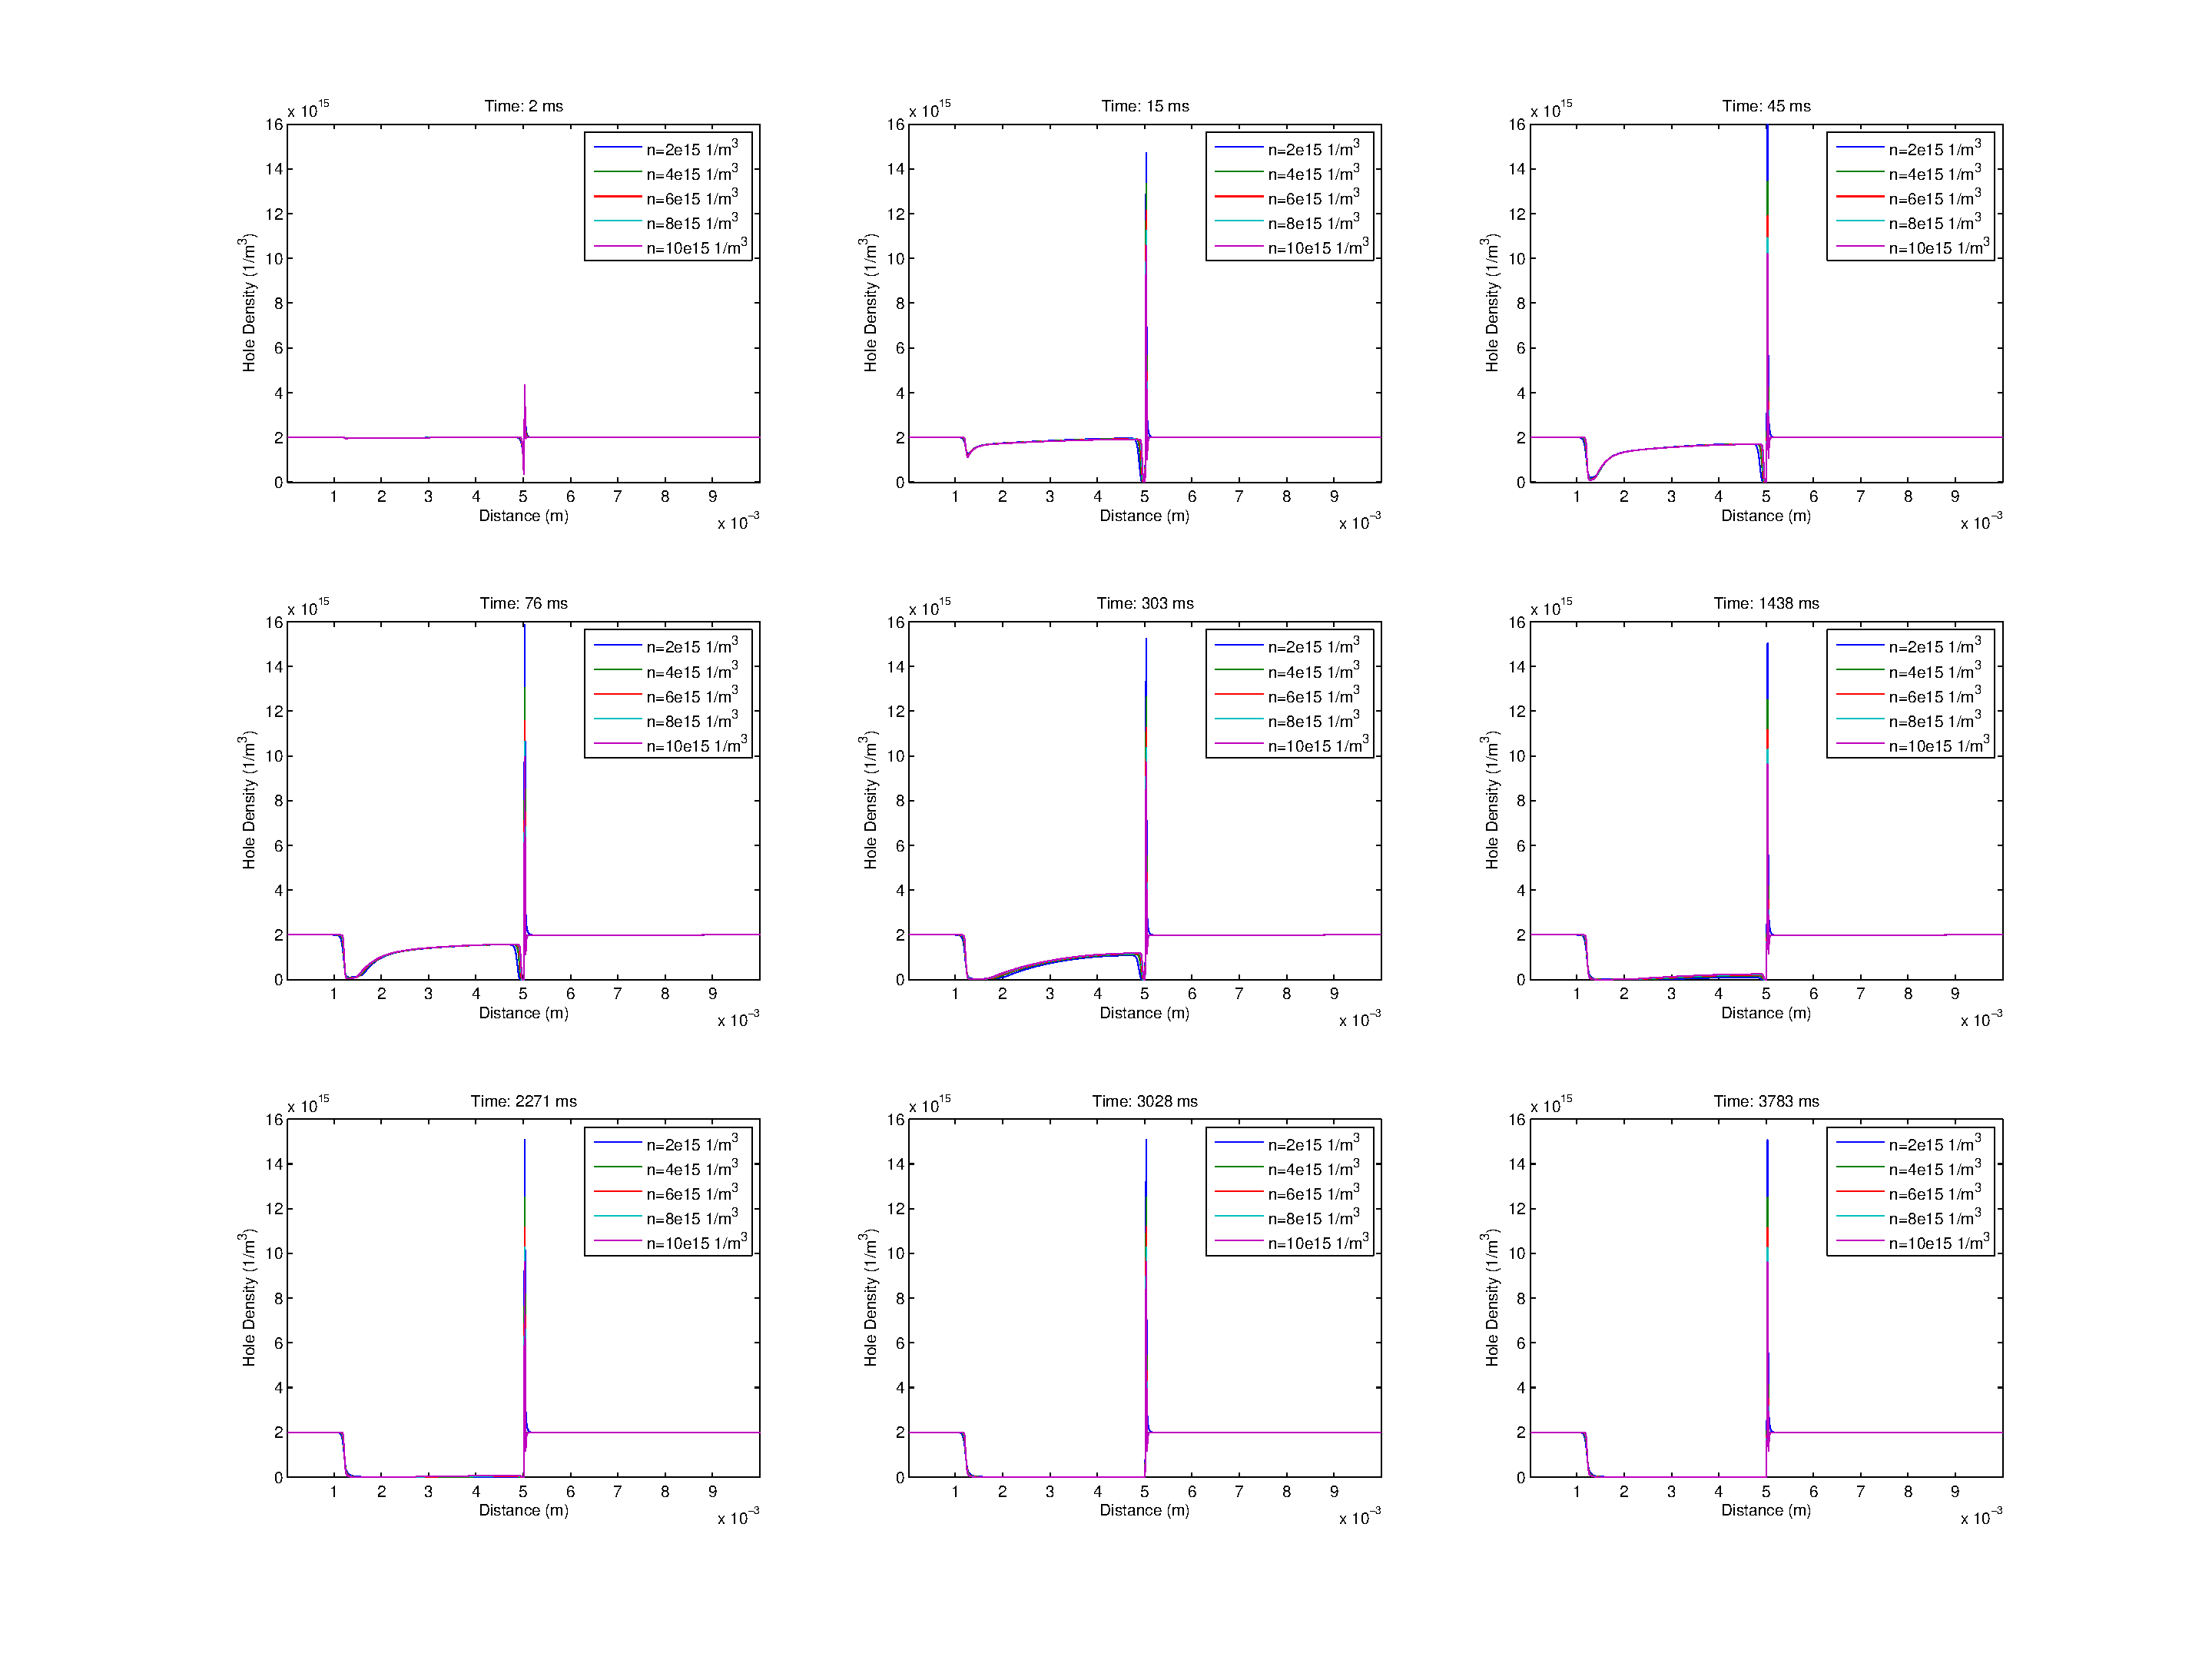
\includegraphics[scale=0.40]{Ex5Hole_Notch_Time1}
\caption{Normalized hole distribution over time} 
\label{}
\end{figure}
\end{landscape}


\begin{landscape}
\begin{figure}[!htp]
\centering
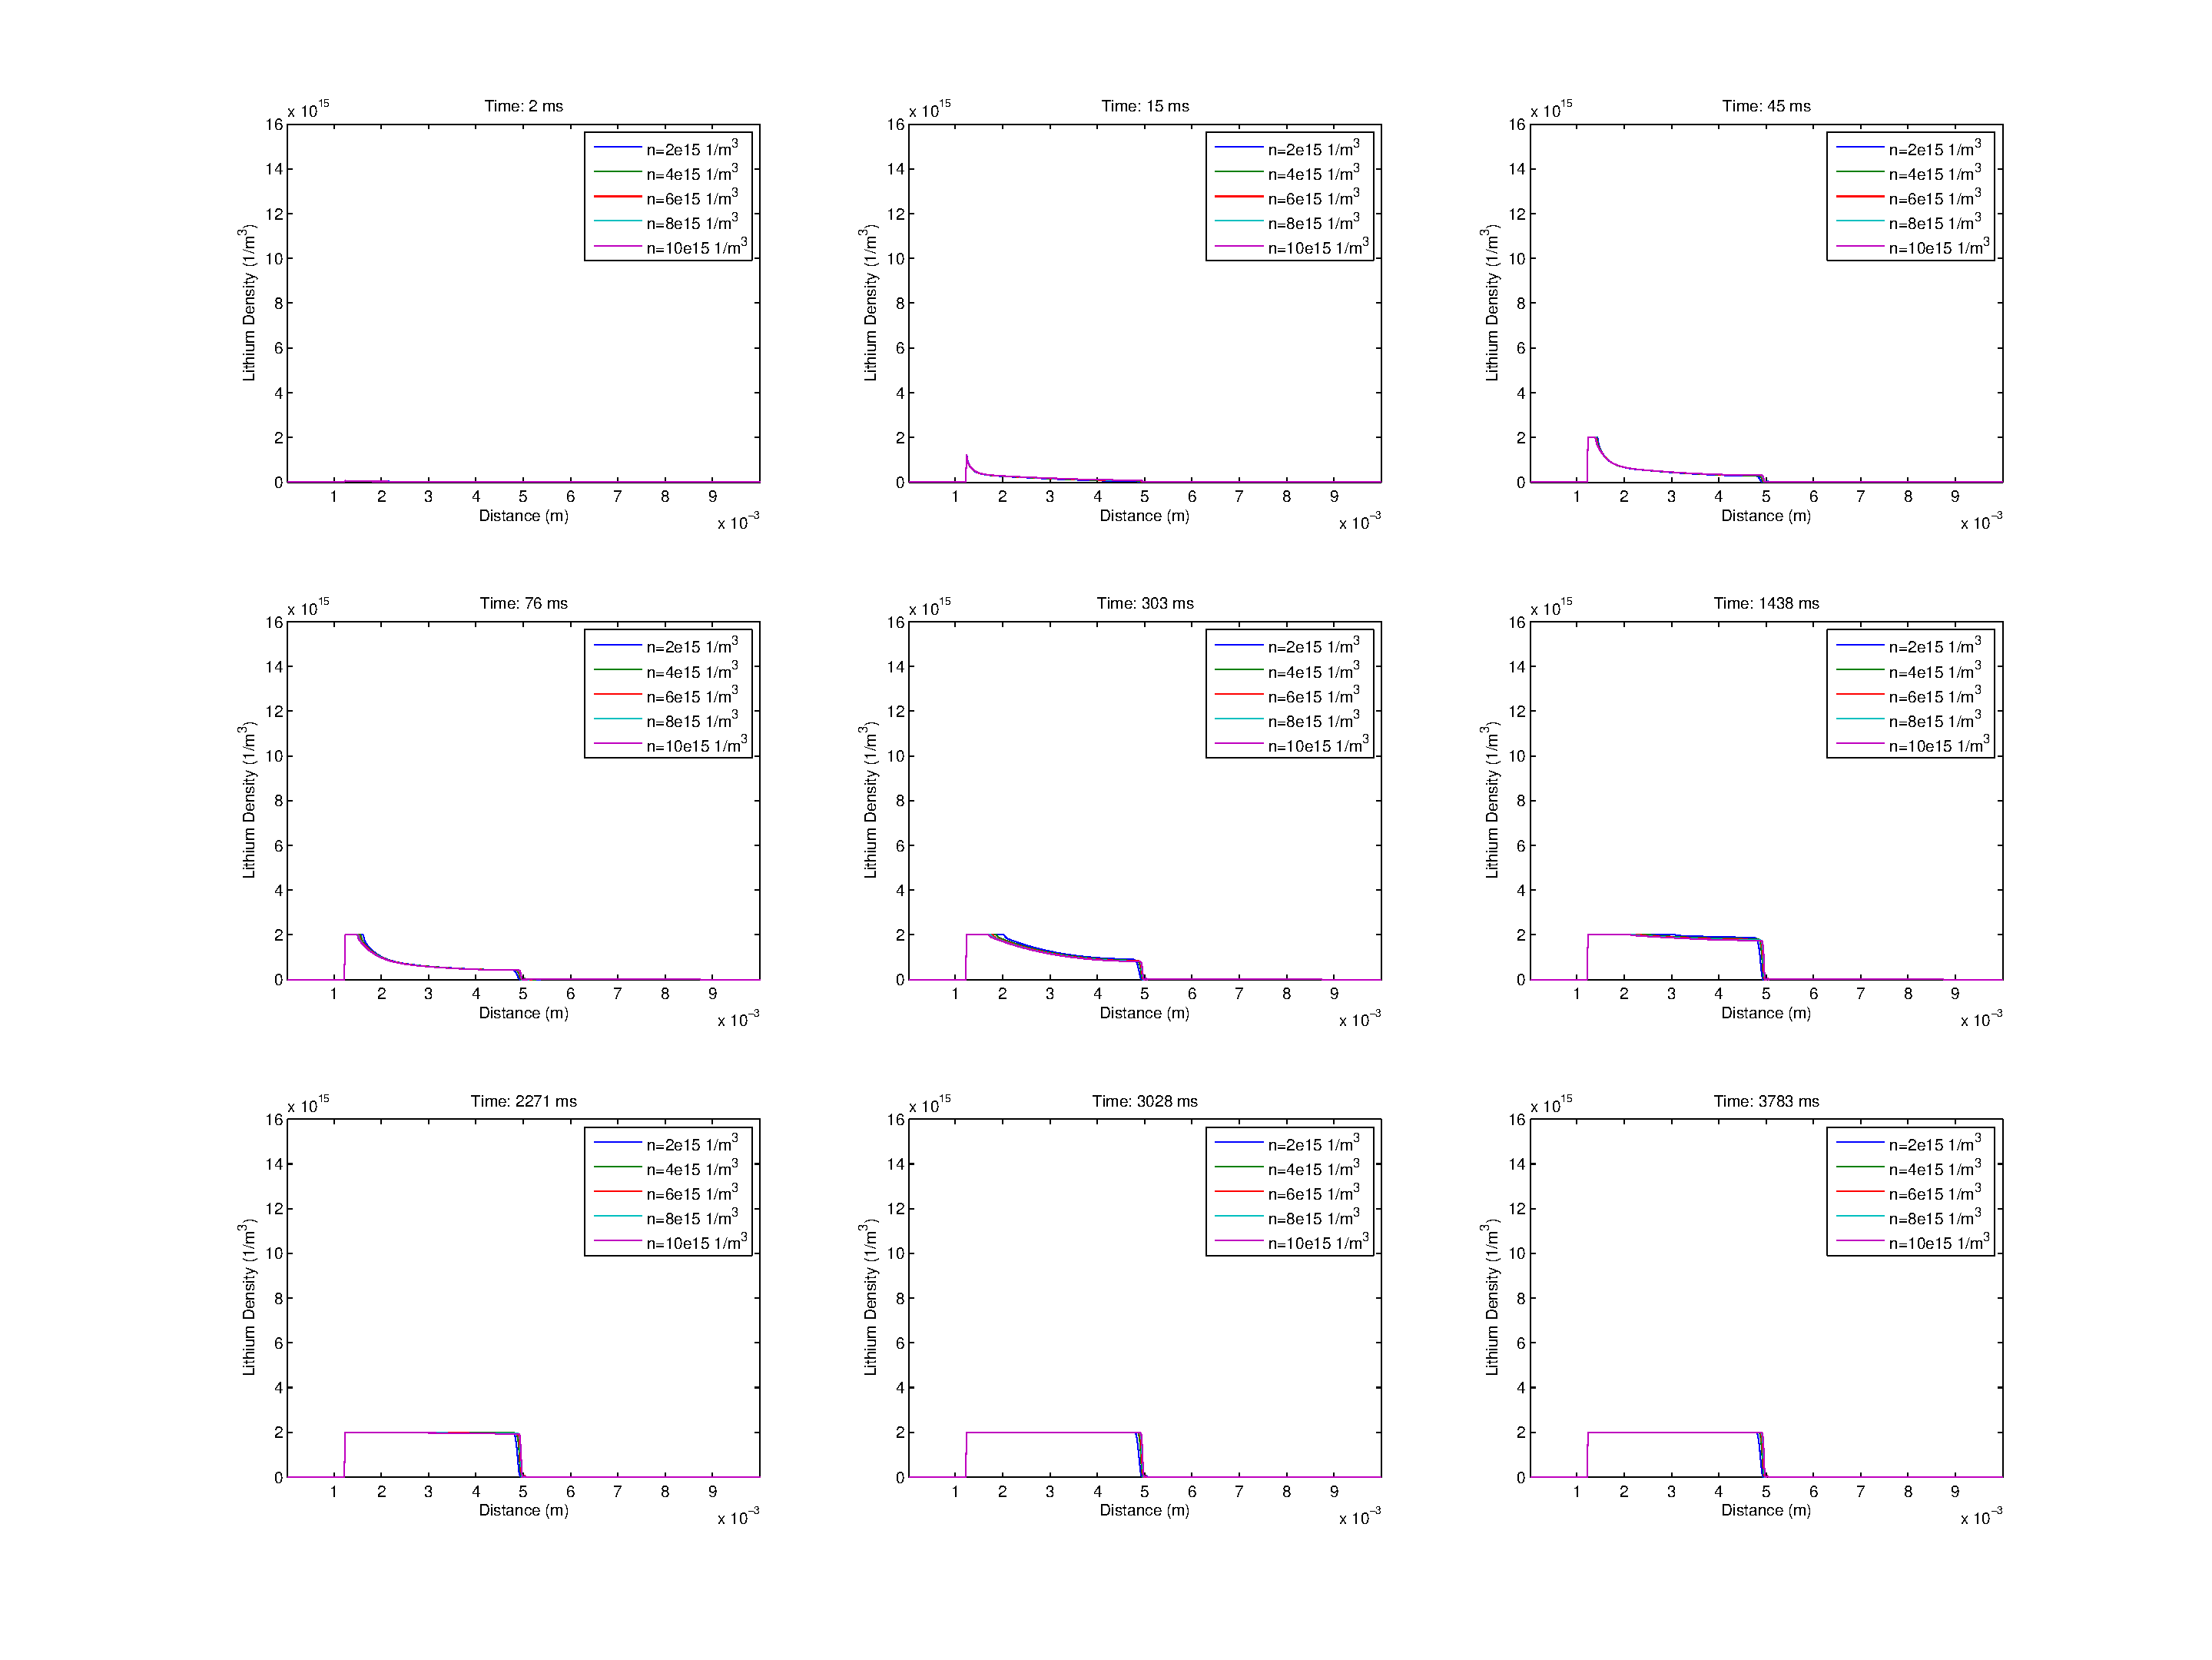
\includegraphics[scale=0.40]{Ex5Li_Notch_Time1}
\caption{Normalized lithium distribution over time} 
\label{}
\end{figure}
\end{landscape}


\begin{landscape}
\begin{figure}[!htp]
\centering
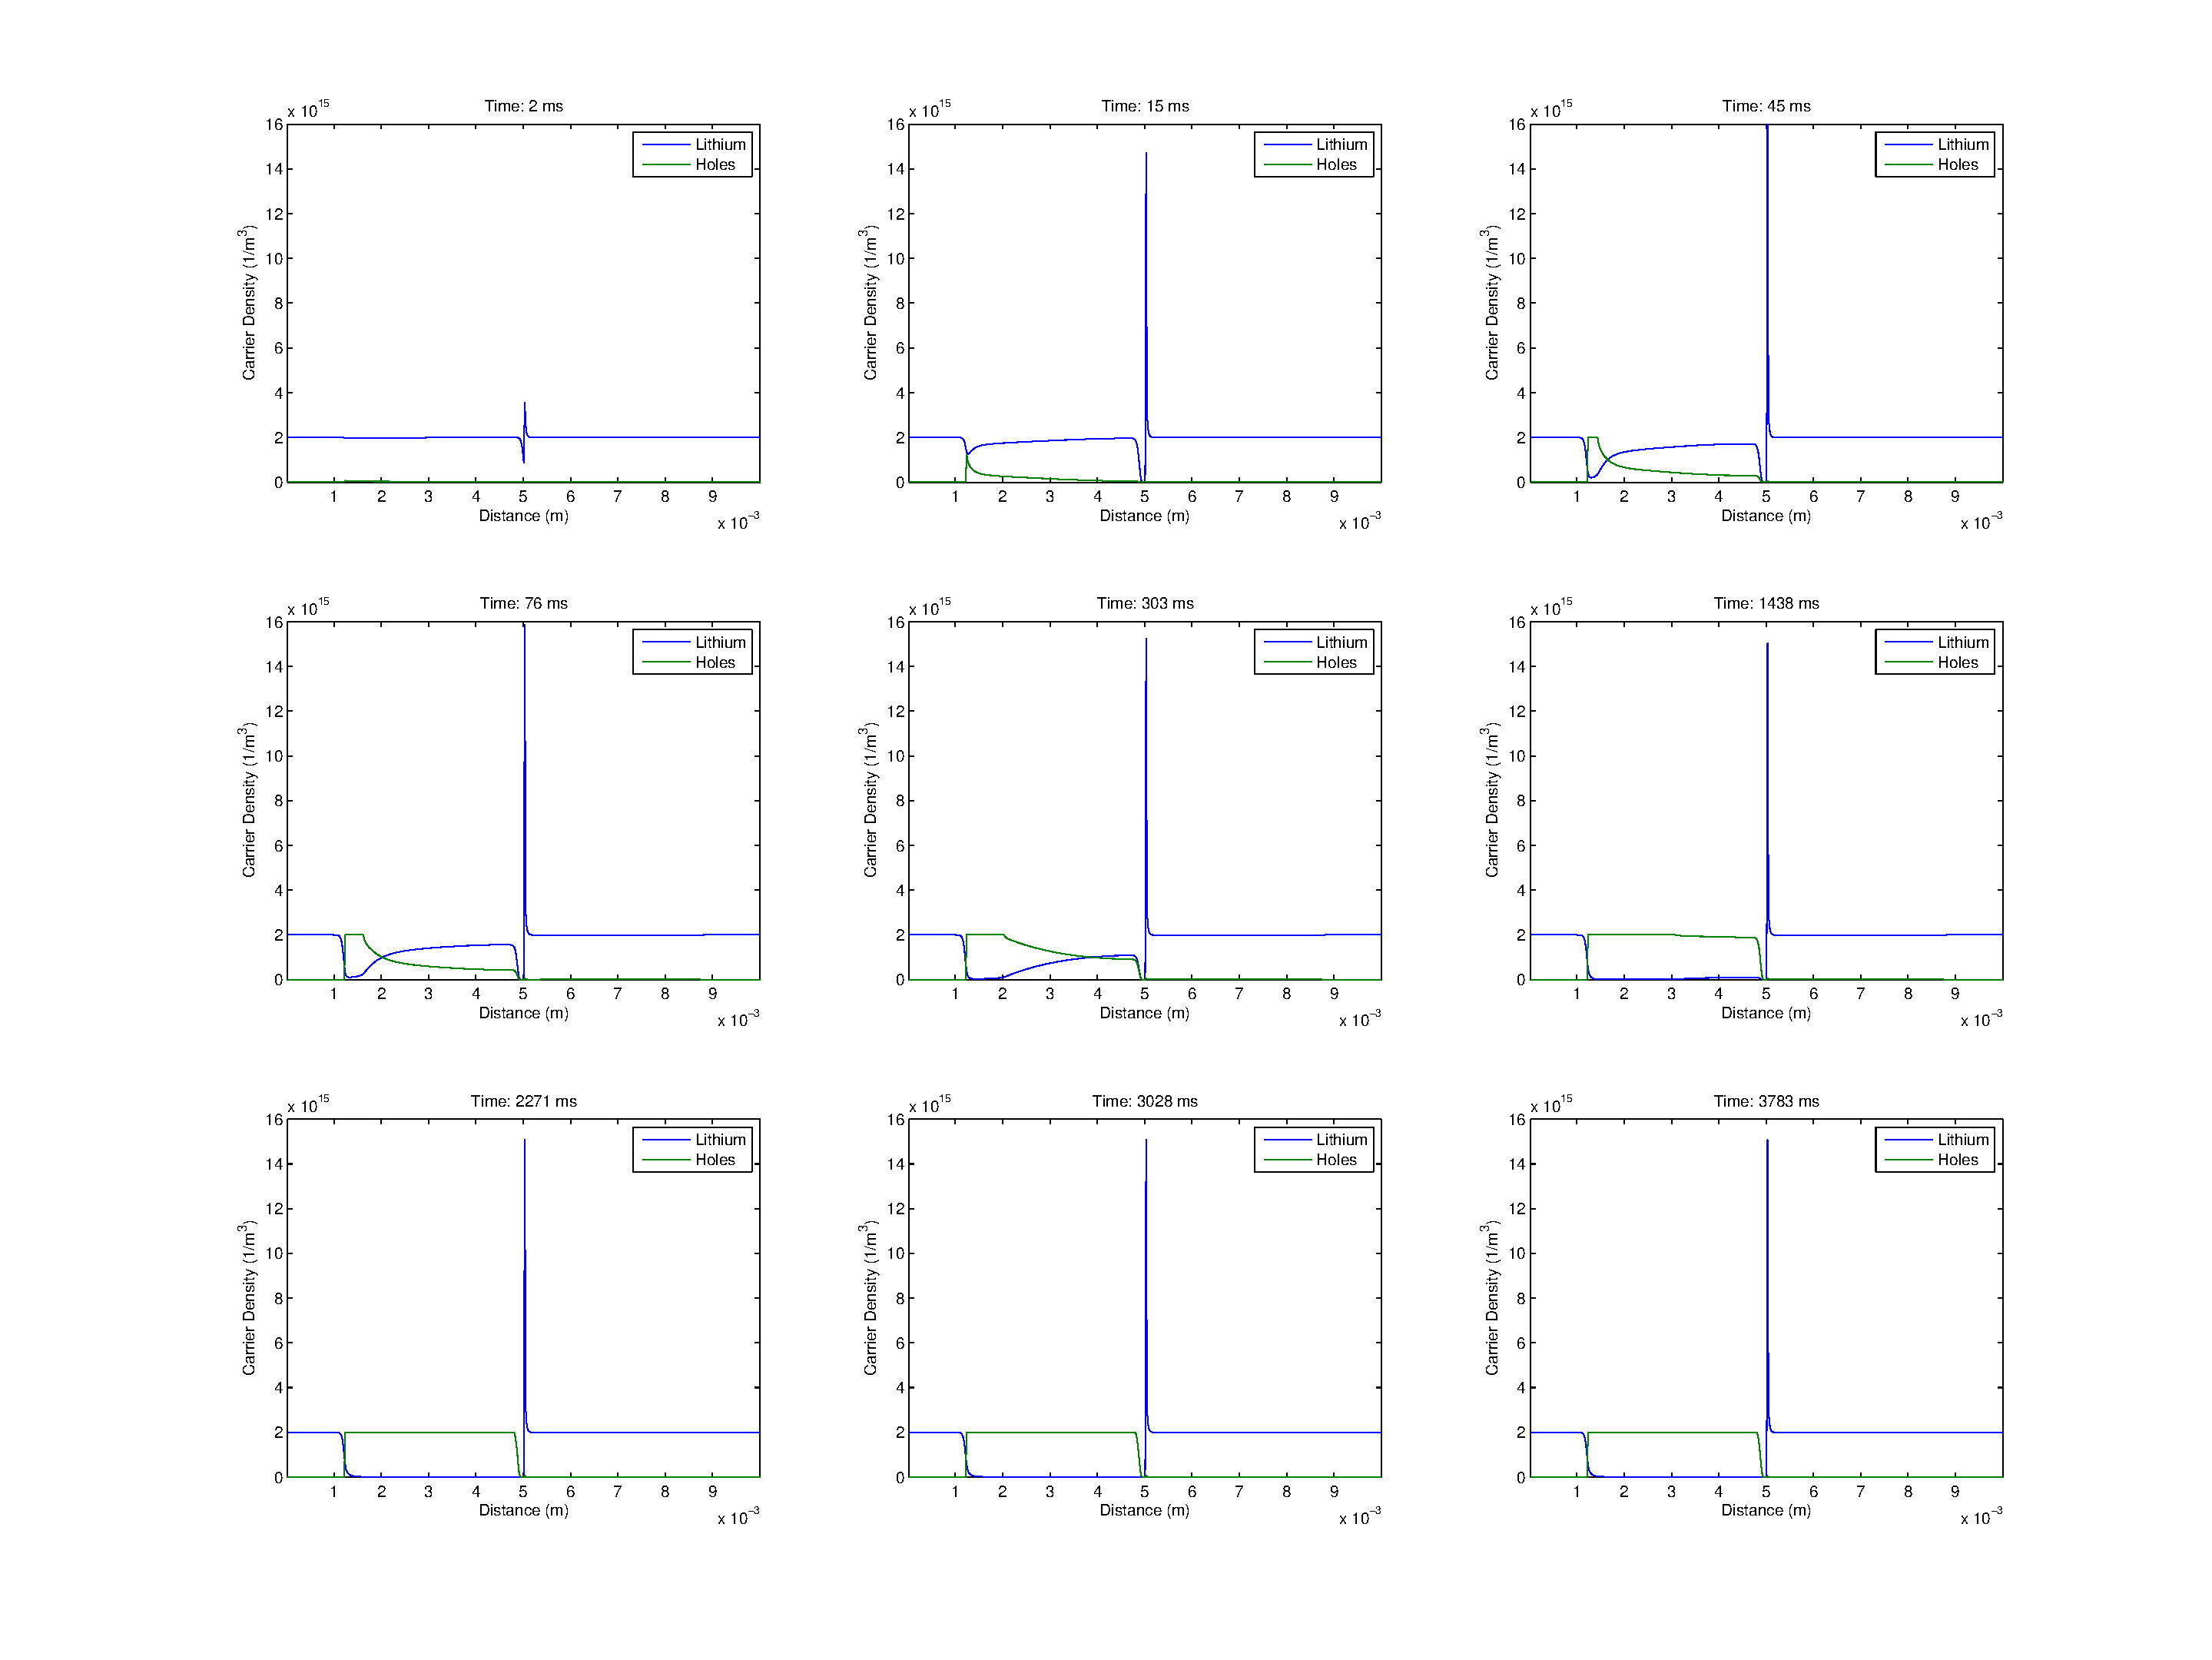
\includegraphics[scale=0.40]{Ex5Lip_Notch_Time1}
\caption{Lithium and hole distribution over time} 
\label{}
\end{figure}
\end{landscape}


\clearpage
\subsection{Electrolyte/PEDOT Interface (Cross Section 3) }

\begin{landscape}
\begin{figure}[!htp]
\centering
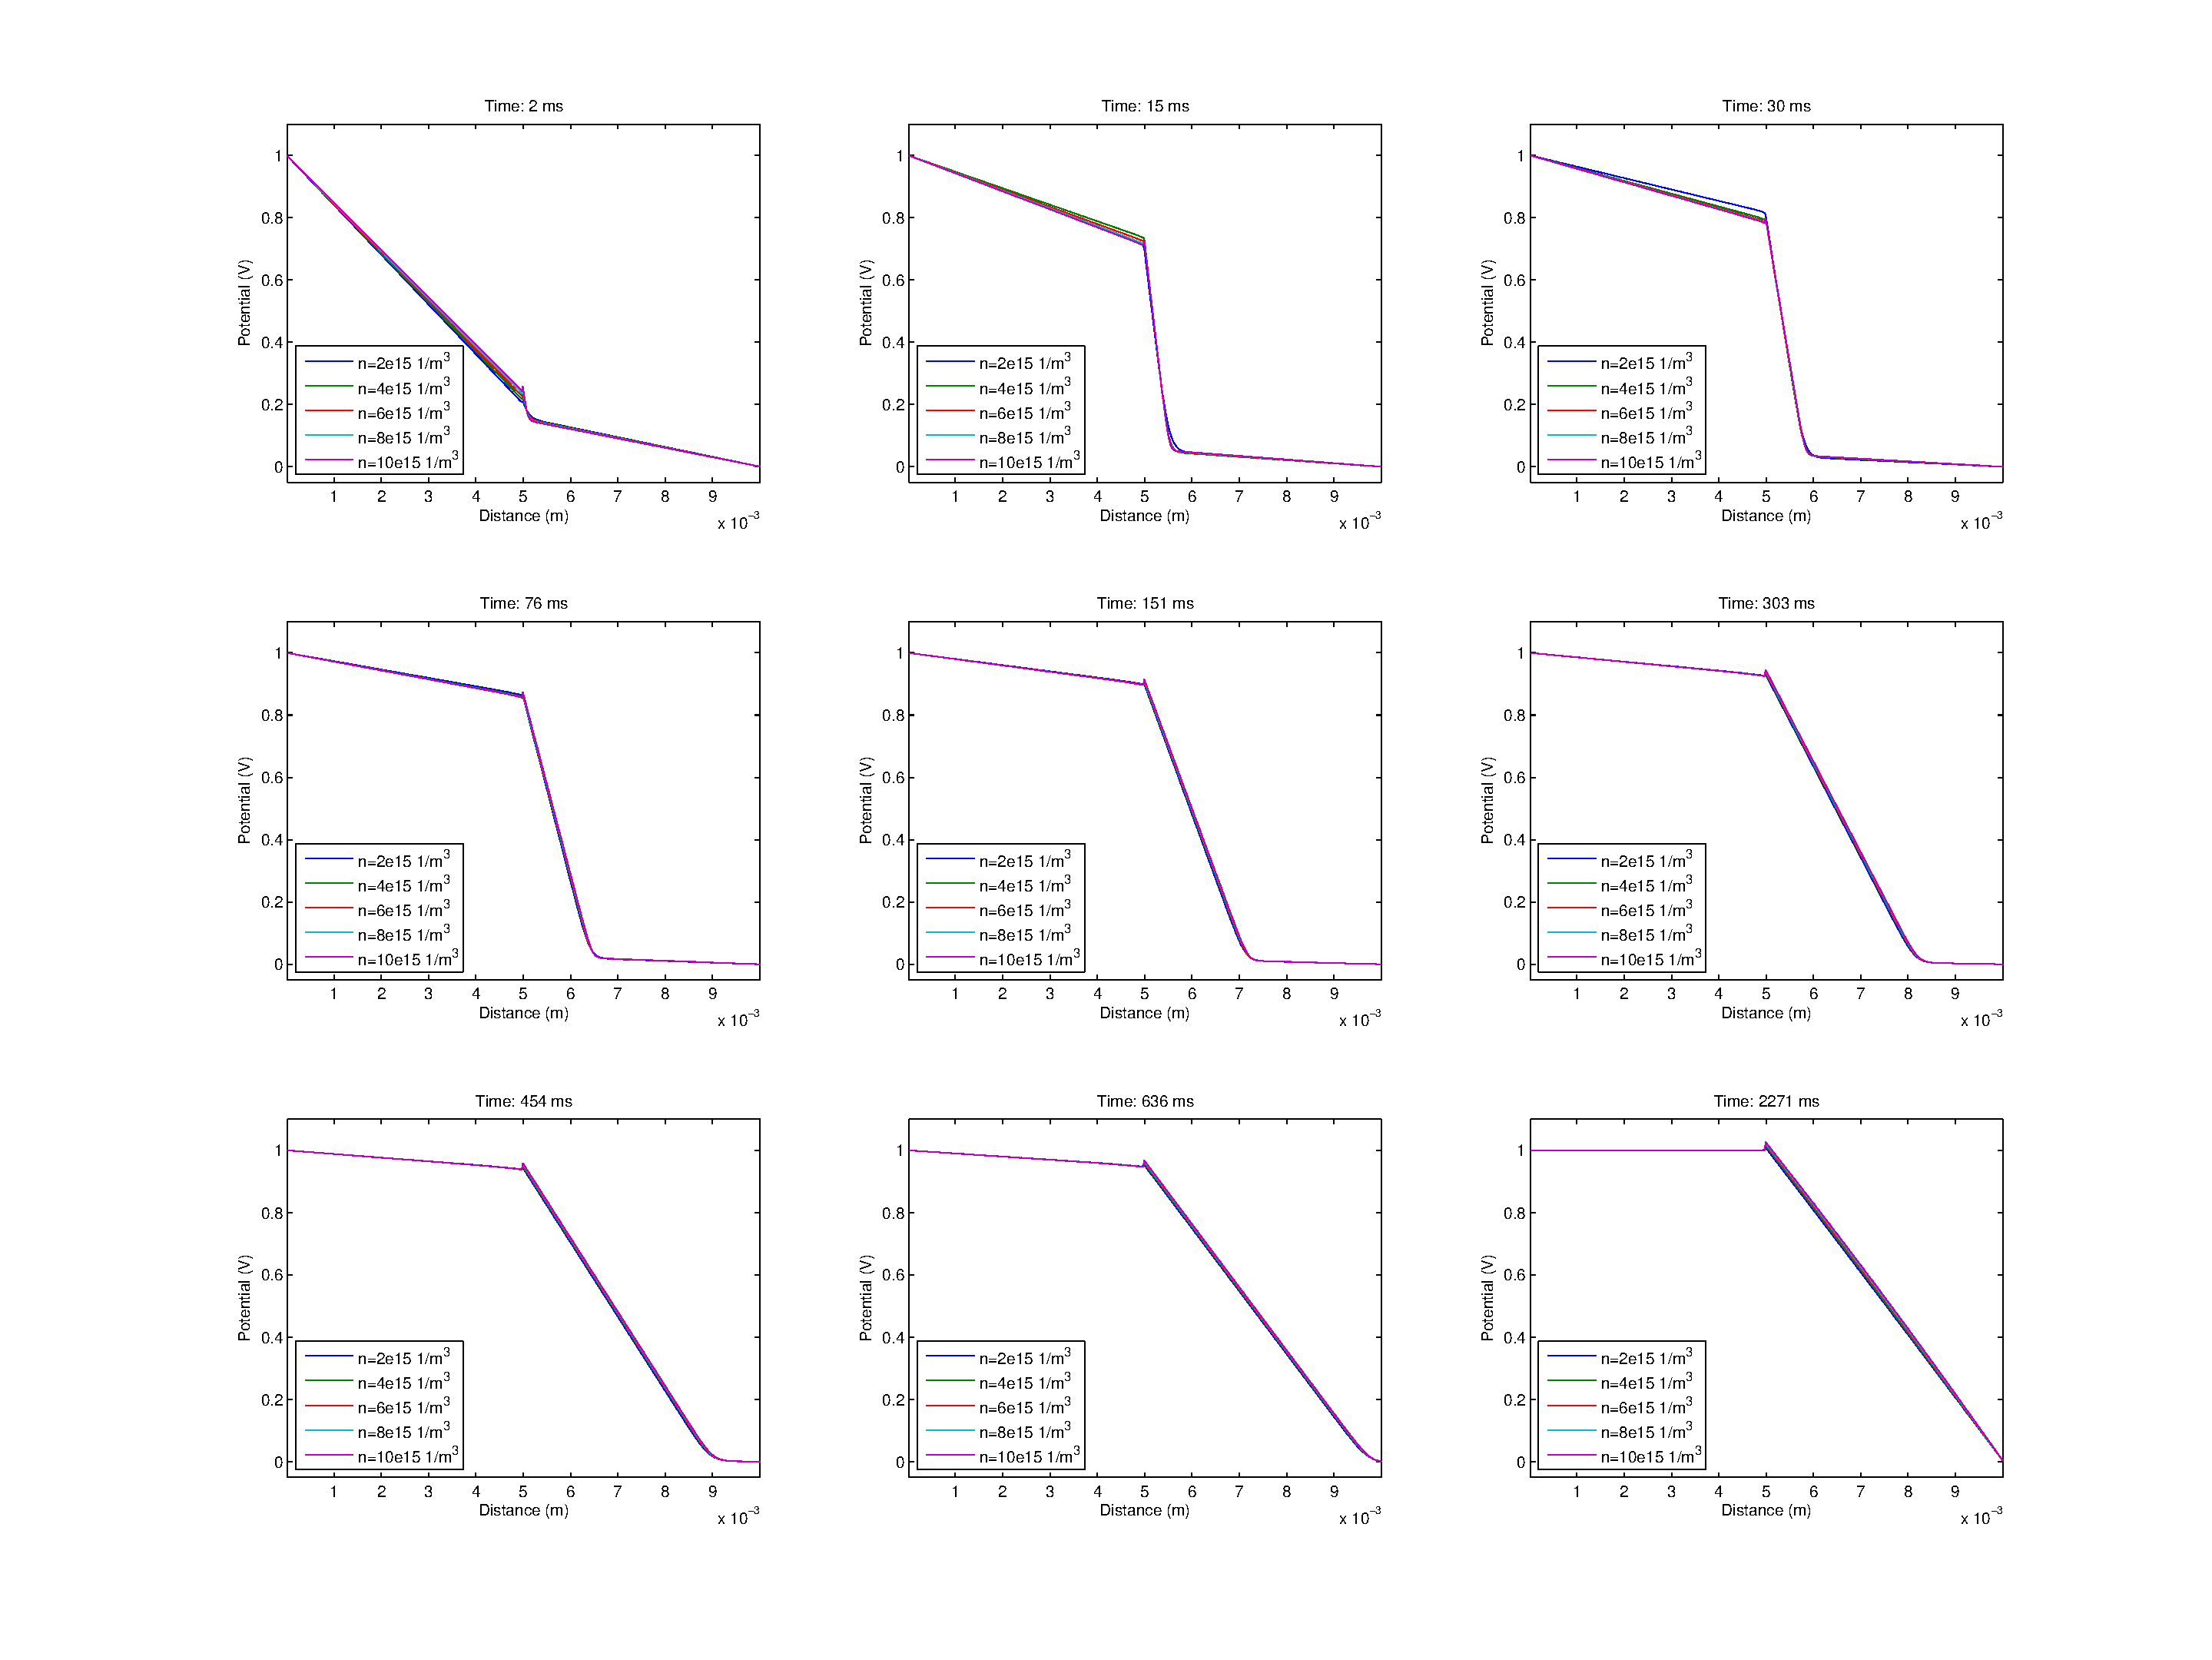
\includegraphics[scale=0.40]{Ex4V_Time}
\caption{Electrolyte/PEDOT interface potential distribution over time} 
\label{}
\end{figure}
\end{landscape}


\begin{landscape}
\begin{figure}[!htp]
\centering
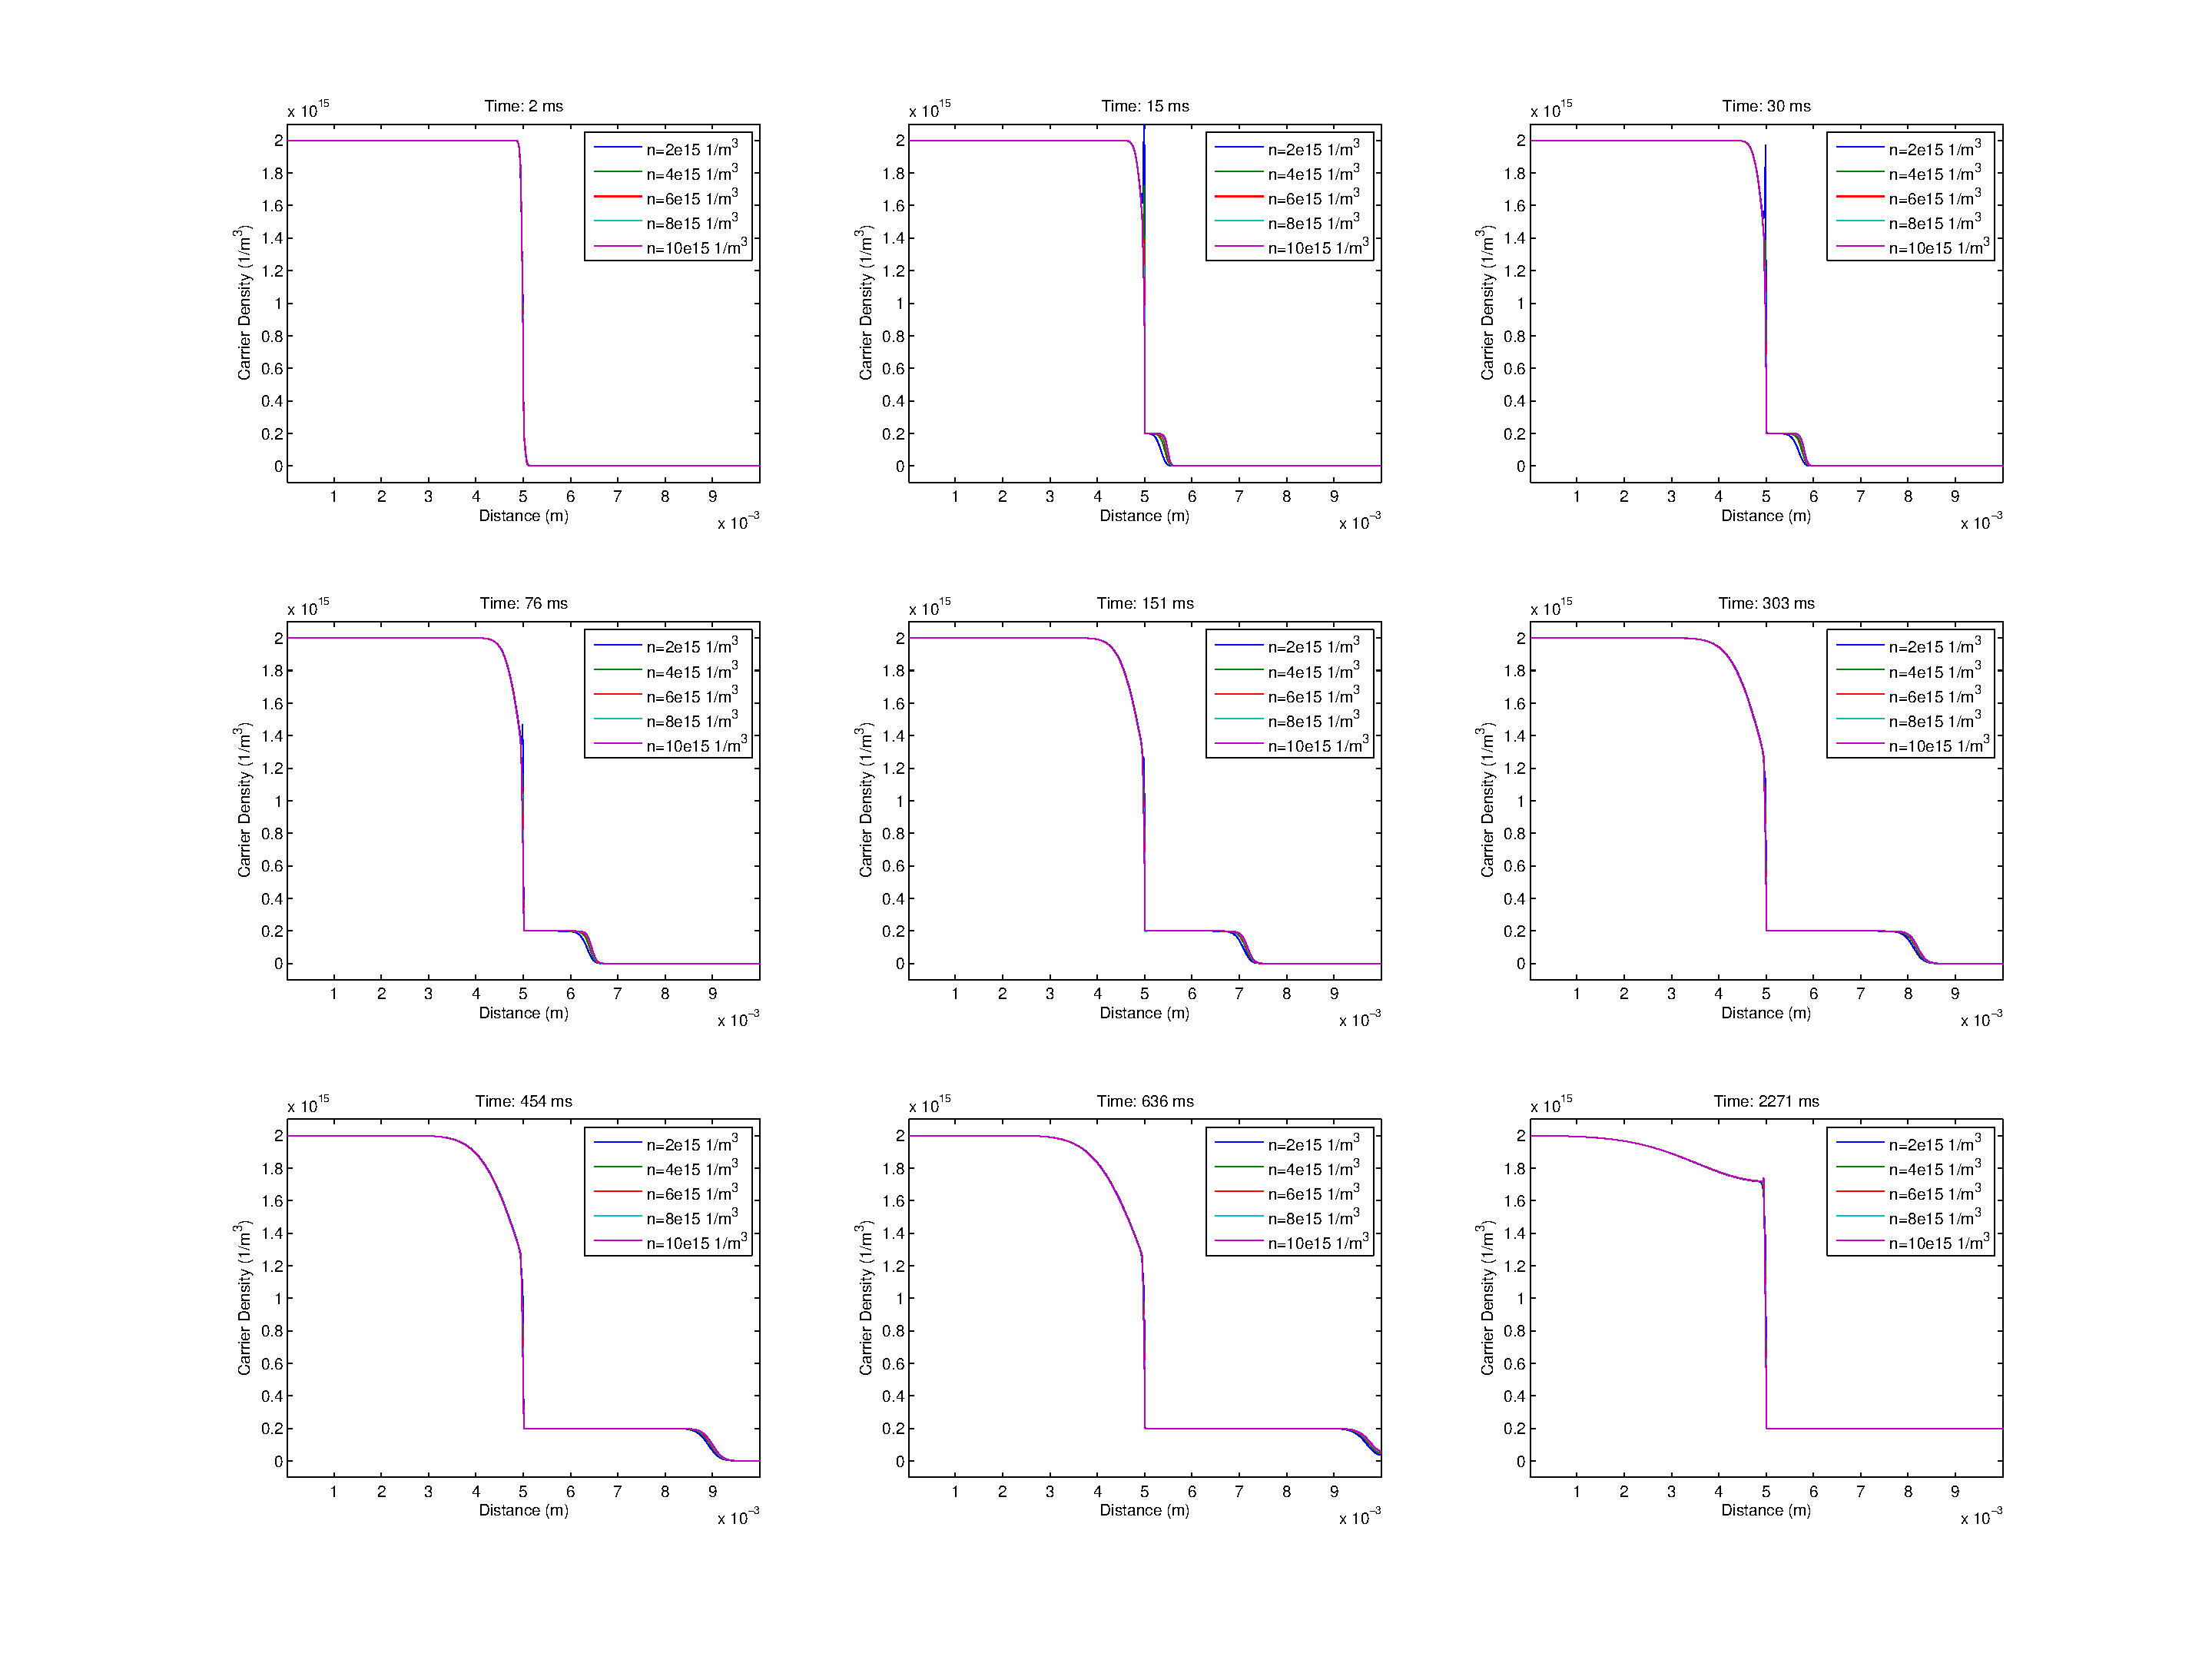
\includegraphics[scale=0.40]{Ex4Np_Time}
\caption{Normalized lithium distribution over time} 
\label{}
\end{figure}
\end{landscape}

\begin{landscape}
\begin{figure}[!htp]
\centering
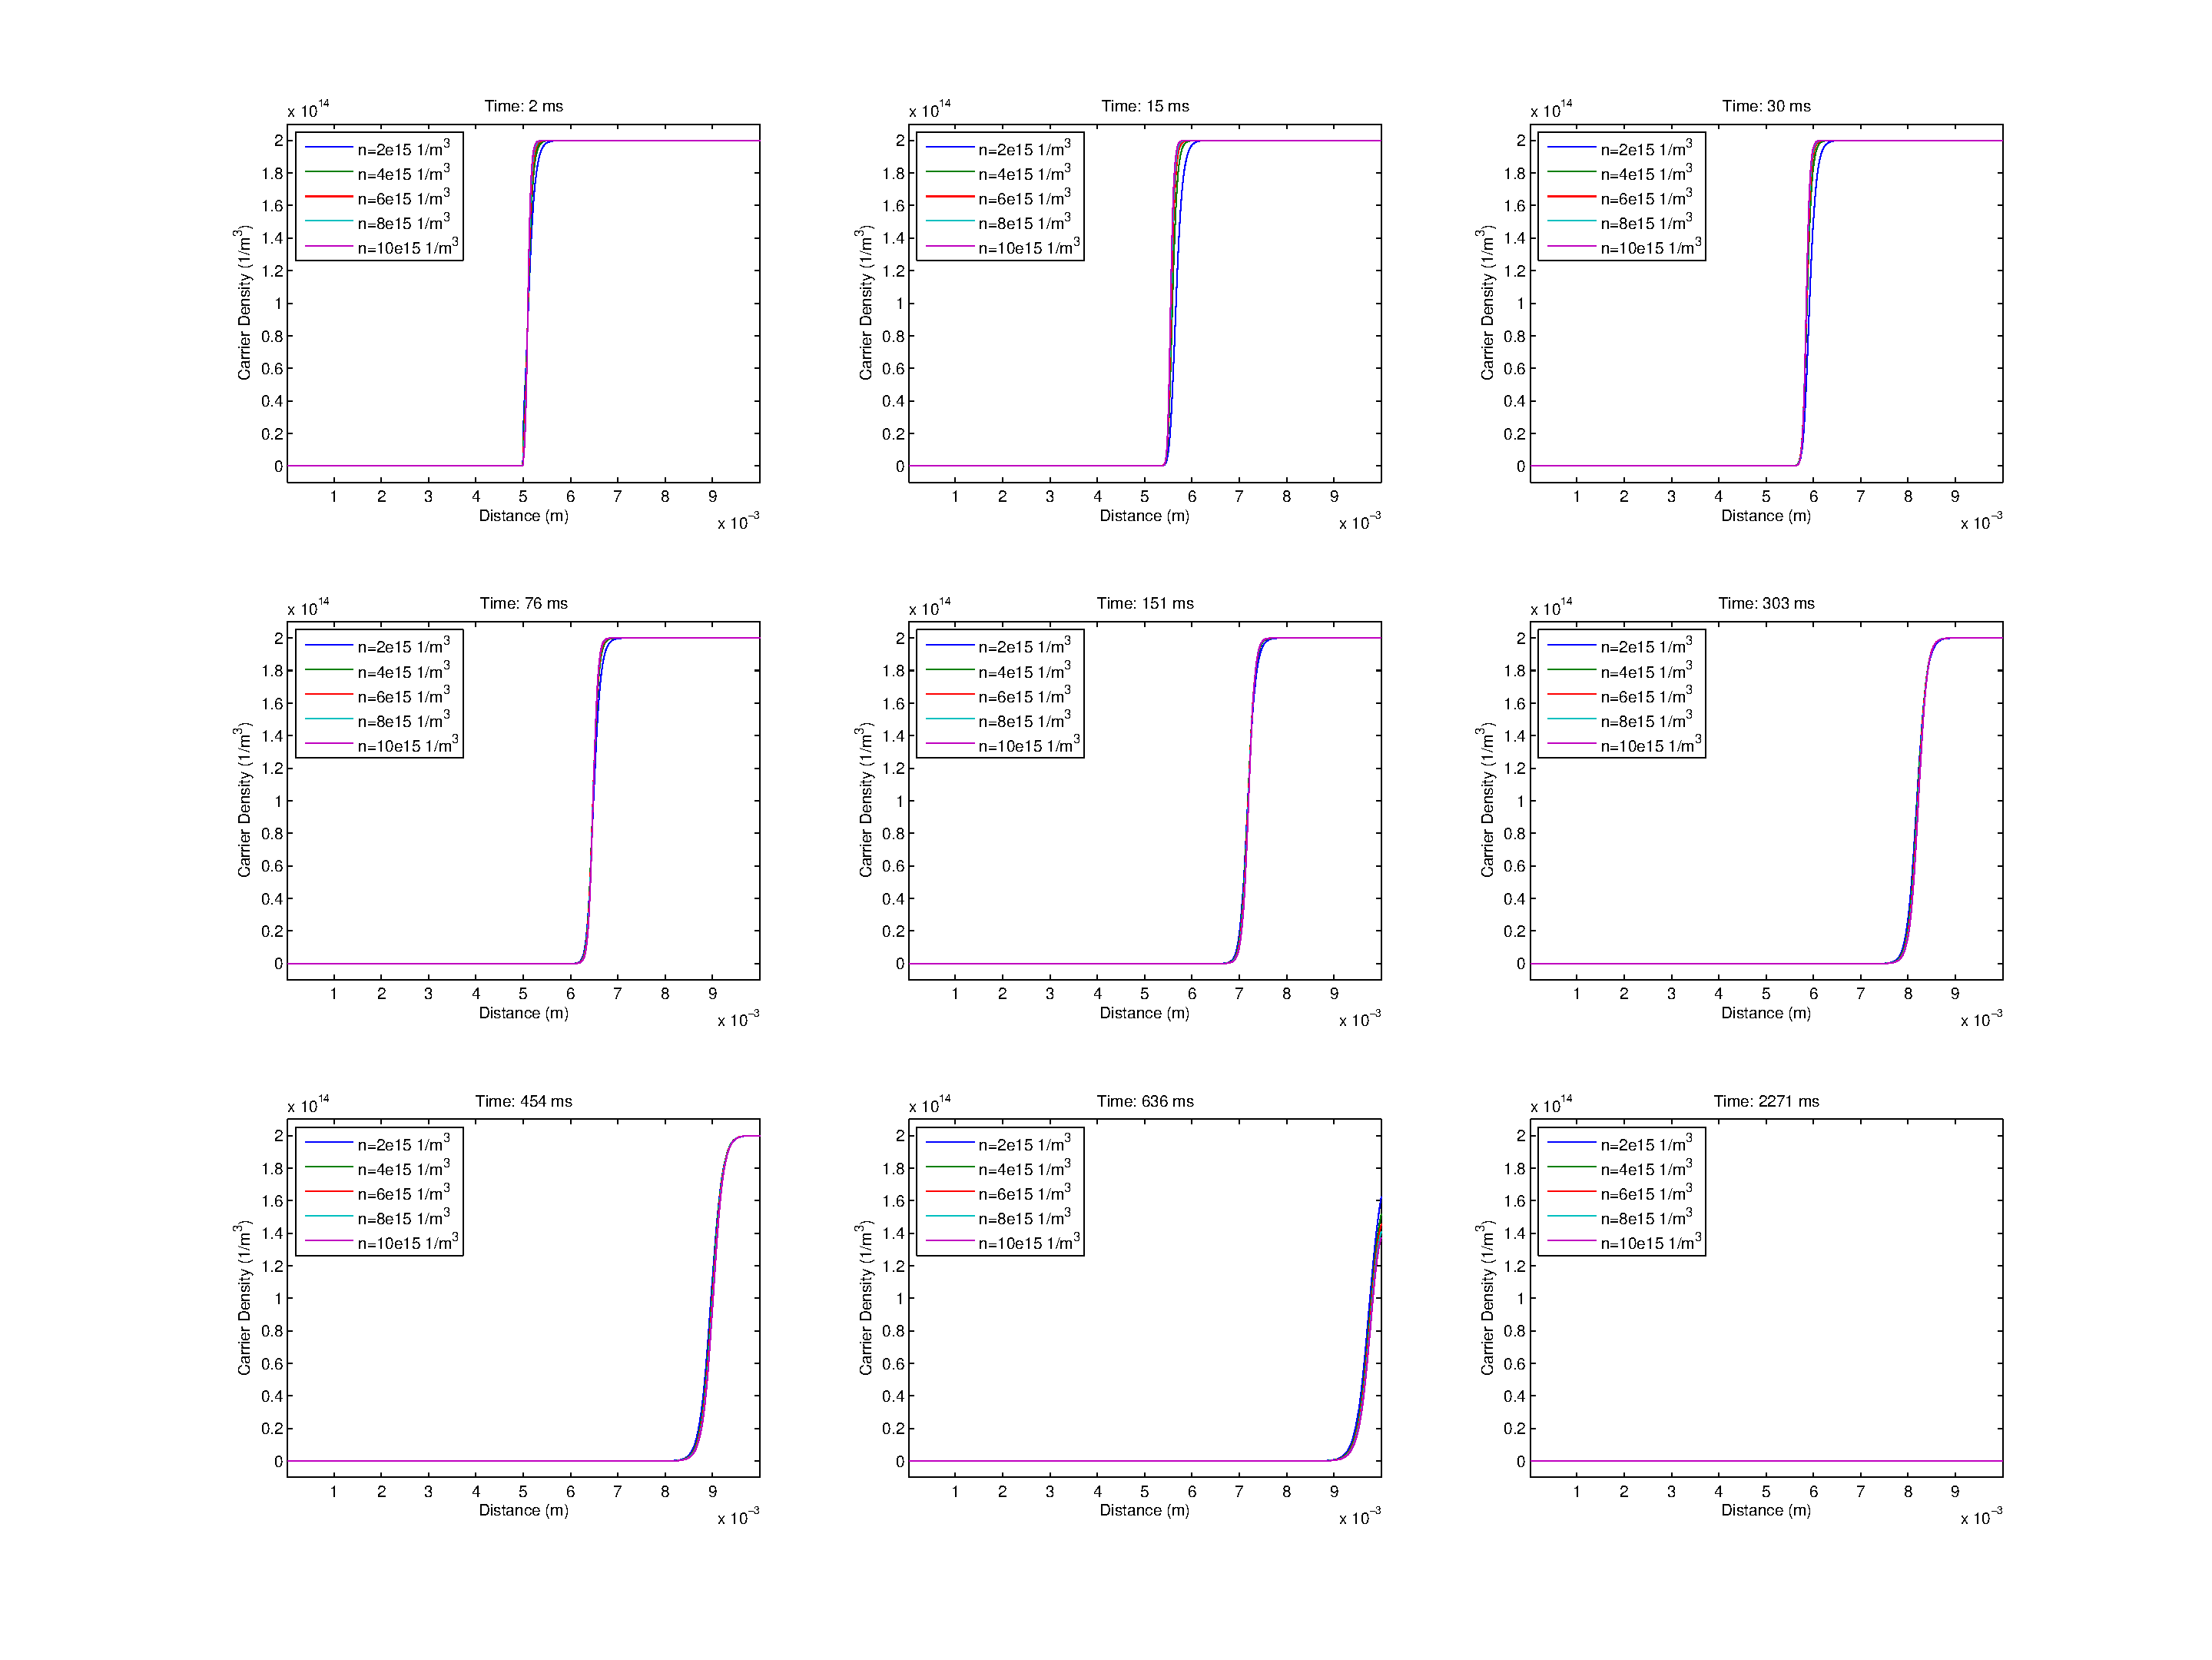
\includegraphics[scale=0.40]{Ex4p_Time}
\caption{Normalized hole distribution over time} 
\label{}
\end{figure}
\end{landscape}

\begin{landscape}
\begin{figure}[!htp]
\centering
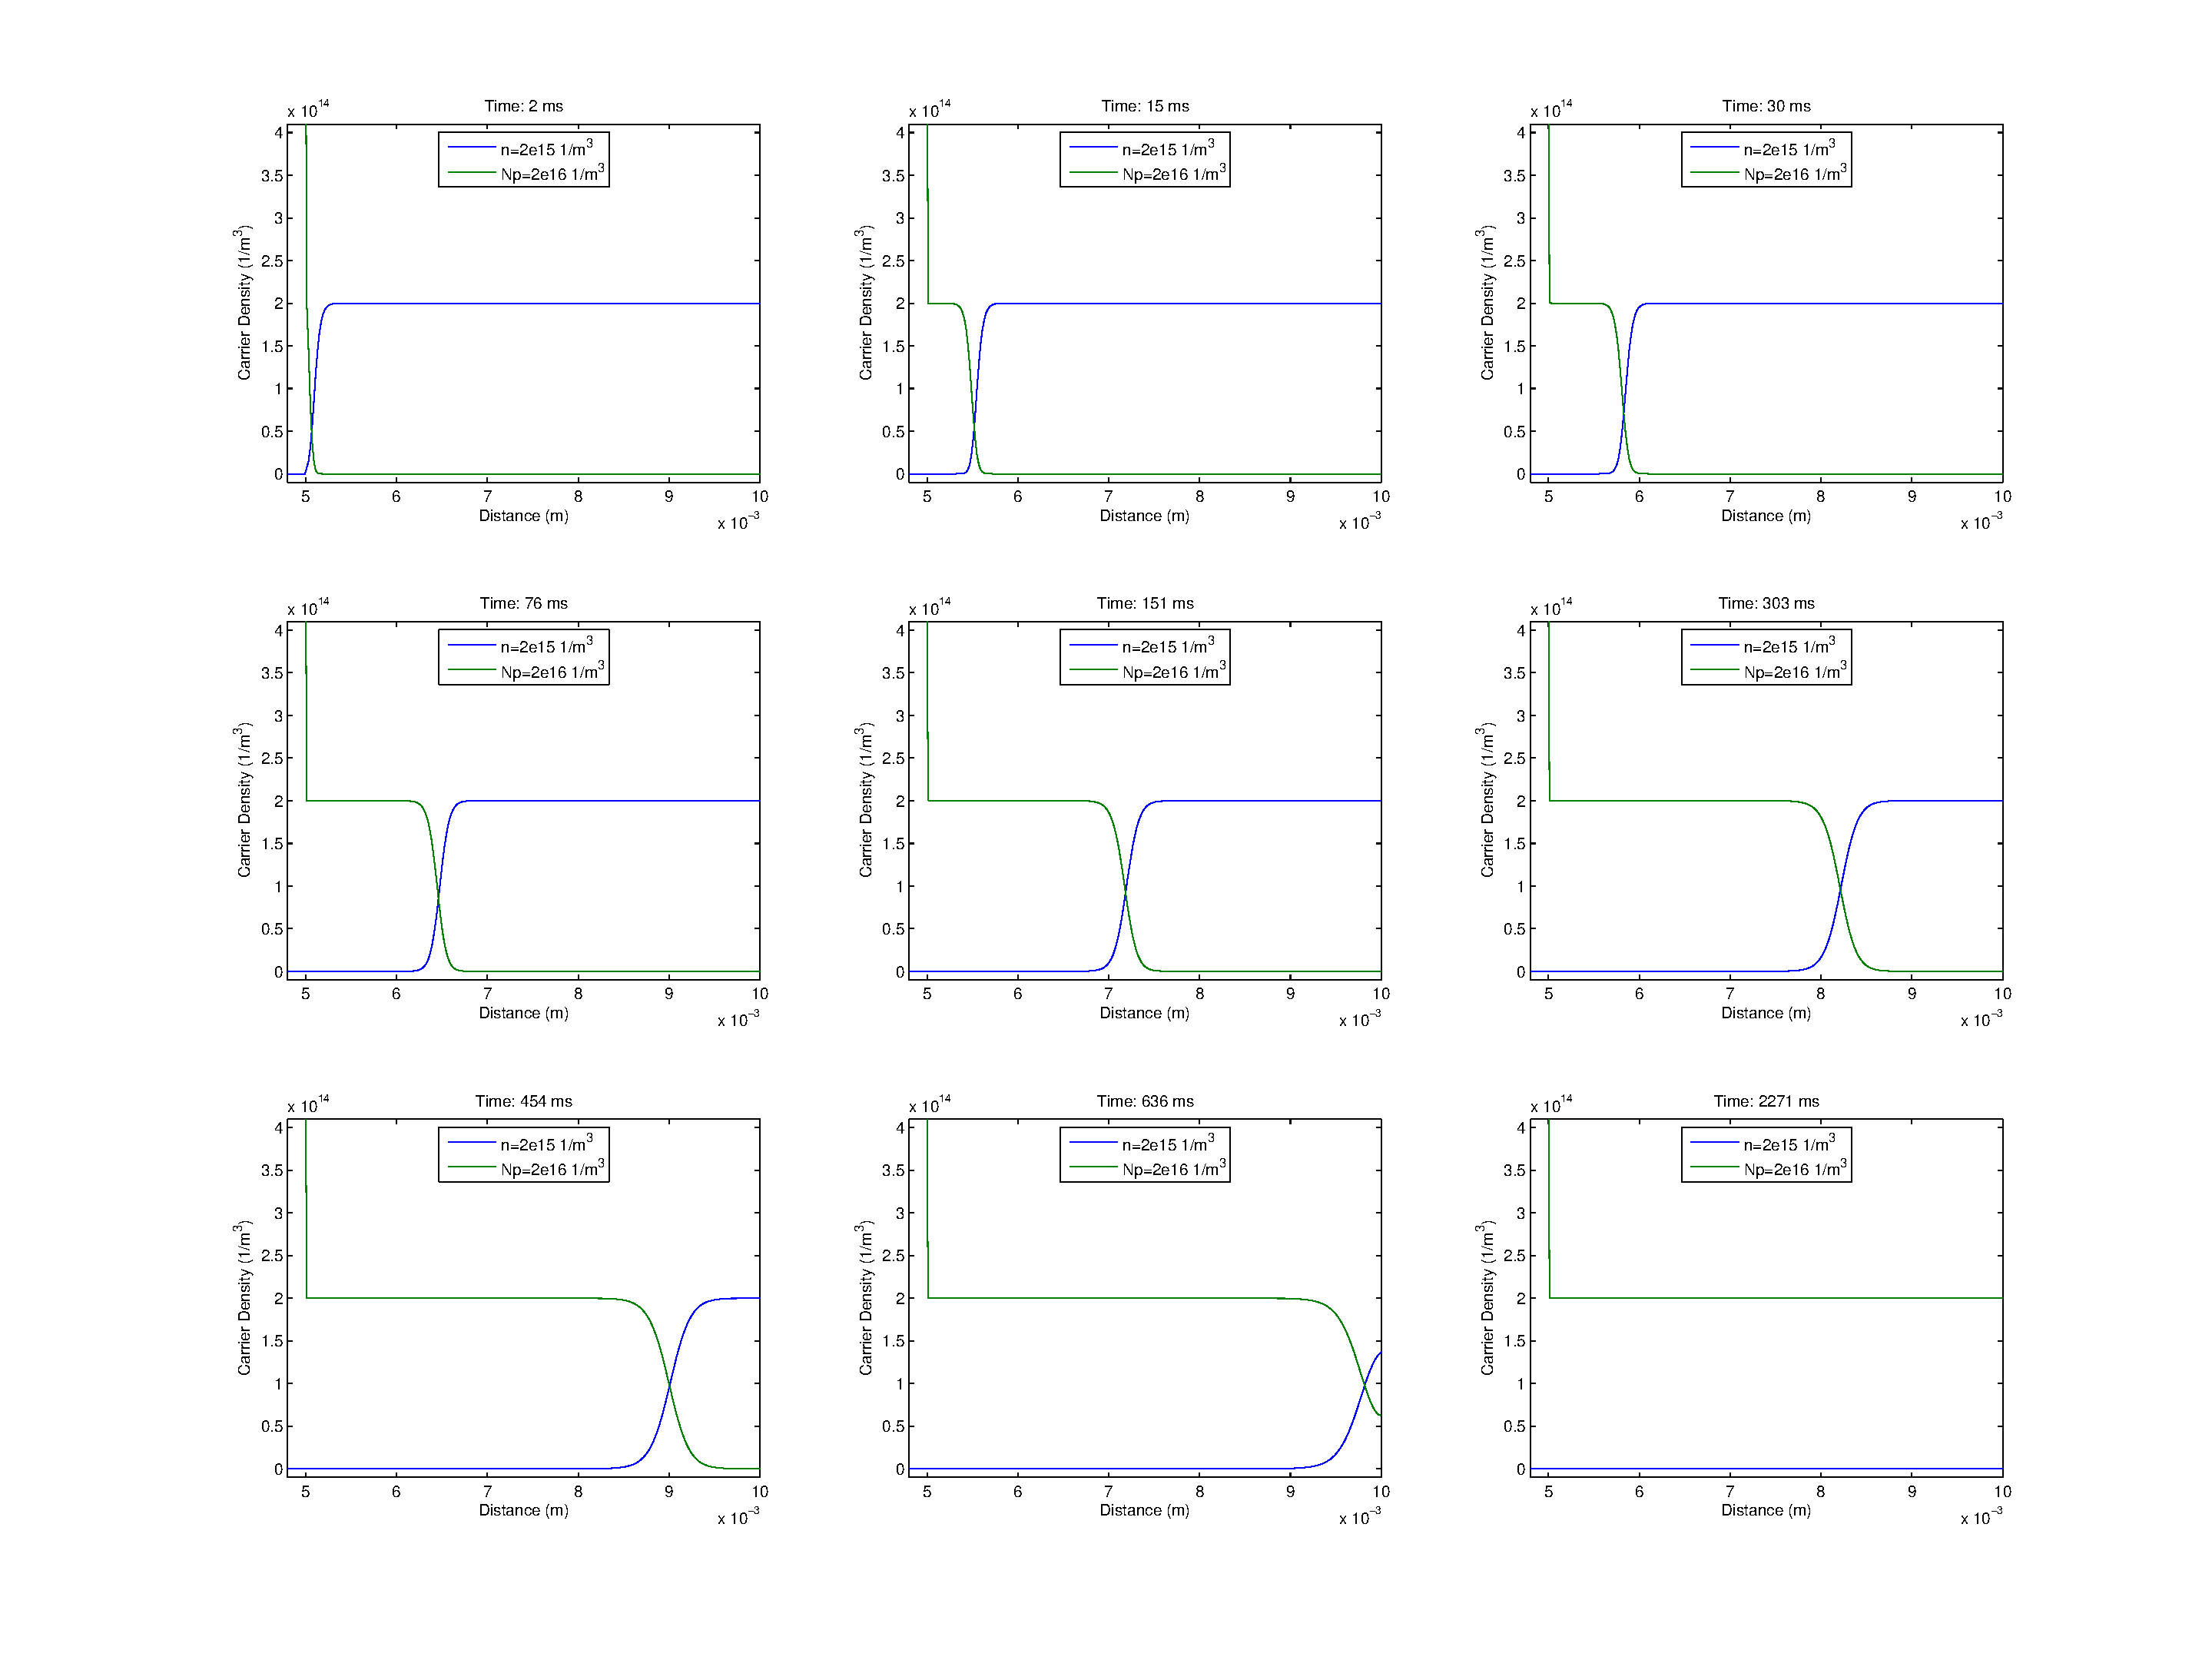
\includegraphics[scale=0.40]{Ex4pNp_Time}
\caption{Lithium and hole distribution over time} 
\label{}
\end{figure}
\end{landscape}






%1-D Vertical Medium and high concentration (hole freeze,# of holes over time)
%1-D Horizontal medium and high concentration (Add memristor pictures,hole freeze,# of holes over time)
